% ----------------------------------------------------------------------
%              Latex TFG plantilla para la Universidad de Cádiz
% ----------------------------------------------------------------------


%: Fichero estilo para Latex

\documentclass[twoside,11pt]{TFGucaPDF}
\usepackage{amsthm}
\usepackage{tcolorbox}
\usepackage{cancel}
\providecommand{\abs}[1]{\lvert#1\rvert}
\providecommand{\norm}[1]{\lVert#1\rVert}
\newcommand{\name}{\mbox{asdfa}\xspace}
%para las definiciones
\newtcolorbox[auto counter, number within=section]{definicion1}[2][]
{fonttitle=\bfseries, title=DEFINICIÓN~\thetcbcounter: #2,#1}
%para los teoremas
\newtcolorbox[auto counter, number within=section]{teorema1}[2][]
{fonttitle=\bfseries, title=TEOREMA~\thetcbcounter: #2,#1}
\newtcolorbox[auto counter, number within=section]{proposicion1}[2][]
{fonttitle=\bfseries, title=PROPOSICION~\thetcbcounter: #2,#1}
\newtcolorbox[auto counter, number within=section]{lema1}[2][]
{fonttitle=\bfseries, title=Lema~\thetcbcounter: #2,#1}


%para los corolarios
\newtcolorbox[auto counter, number within=section]{corolario1}[2][]
{fonttitle=\bfseries, title=COROLARIO~\thetcbcounter: #2,#1}
\usepackage[spanish]{babel}

%: Fichero de macros para Latex

\def\IR{\ensuremath{\mathbb R}}
\def\IK{\ensuremath{\mathbb K}}
\def\IC{\ensuremath{\mathbb C}}
\def\IN{\ensuremath{\mathbb N}}
\def\IZ{\ensuremath{\mathbb Z}}
\def\IQ{\ensuremath{\mathbb Q}}
\def\IA{\ensuremath{\mathbb A}}

\def\centra#1{\begin{center} #1\end{center}}

\def\sen{\mathop{\rm sen}\nolimits}
\def\arcsen{\mathop{\rm arcsen}\nolimits}
\def\tg{\mathop{\rm tg}\nolimits}
\def\cotg{\mathop{\rm cotg}\nolimits}
\def\cosec{\mathop{\rm cosec}\nolimits}
\def\arctg{\mathop{\rm arctg}\nolimits}

\def\suma#1#2{\displaystyle\sum_{#1}^{#2}}
\def\fra#1#2{\displaystyle {#1\over #2}}
\def\Lim{\ensuremath{\displaystyle\lim}}

\newcommand{\be}{\begin{enumerate}}
\newcommand{\ee}{\end{enumerate}}

\newcommand{\bi}{\begin{itemize}}
\newcommand{\ei}{\end{itemize}}

\newcommand{\bd}{\begin{description}}
\newcommand{\ed}{\end{description}}

\newcommand{\beq}{\begin{equation}}
\newcommand{\eeq}{\end{equation}}

\newcommand{\braya}{\begin{itemize}\renewcommand{\labelitemi}{\labelitemii}}
\newcommand{\eraya}{\end{itemize}}

\newcommand{\bletra}{\begin{list}{(\alph{enumiii})}{\usecounter{enumiii}}}
\newcommand{\eletra}{\end{list}}

\newcommand{\broman}{\begin{list}{(\roman{enumiii})}{\usecounter{enumiii}}}
\newcommand{\eroman}{\end{list}}

\newcommand{\bRoman}{\begin{list}{(\Roman{enumi})}{\usecounter{enumi}}}
\newcommand{\eRoman}{\end{list}}

\def\xn{(x_1,x_2,\ldots ,x_n)}
\def\yn{(y_1,y_2,\ldots ,y_n)}
\def\xm{(x_1,x_2,\ldots ,x_m)}
\def\ym{(y_1,y_2,\ldots ,y_m)}

\def\caja{\hspace*{\fill}$\Box$}

\def\nveces#1{\matrix{\mathop{\frown}\limits^{#1}
\cr \cdots\cr \mbox{}} }

\def\Veces#1{\buildrel {\buildrel #1\over\frown} \over\cdots}

\def\sucesion#1#2{\left(#1_#2\right)_#2}




%: ----------------------------------------------------------------------
%:                  PORTADA: Nombre, título, ...
% ----------------------------------------------------------------------

    \pdfinfo { /Title  ( Solución numérica de la ecuación de Benjamin-Bona-Mahony-Burgers con el método Galerkin)
               /Creator (TeX)
               /Producer (pdfTeX)
               /Author (Name surname)  %%%%%%%%% XXX    Nombre y apellidos
               /CreationDate (D:DDMMYYYhhmmss)  %format D:YYYYMMDDhhmmss
               /ModDate (D:DDMMYYYhhmm)
               /Subject (xyz)  %%%%%%%%% XXX   Tema
               /Keywords (keyword1, keyword2, keyword3) }  %%%%%%%%% XXX  claves del trabajo
    \pdfcatalog { /PageMode (/UseOutlines)
                  /OpenAction (fitbh)  }


\crest{
\includegraphics[width=3.5cm]{SelloUCA.jpg}}


% ---------------------------------------------        RELLENA CON TUS DATOS
\title{Soluci'on numérica de la ecuación de Benjamin-Bona-Mahony-Burgers} %%%%% XXX   Nombre del trabajo
\author{\LARGE Paola Contero Aiza}    %%%    XXX Nombre y apellidos alumno/a
\textadvisor{Tutor: }          %%% XXX  Poner tutor o tutora según proceda
\advisor{Dr. Rafael de la Rosa Silva}  %%% XXX  Nombre del tutor o tutora
\advisortwo{}                  %%% XXX  Nombre del 2º tutor si lo hay
\textsignaturecandidate{Firma de la alumna}   %%% XXX  Poner alumno o alumna según proceda
\textsignatureadvisor{Firma de la tutor}    %%% XXX  Poner tutor o tutora según proceda
\cityofbirth{Puerto Real, Cádiz}
\degreedate{Septiembre de 2.022}
% ----------------------------------------------------------------------

% Evita los pesados overfull y underfull
\hbadness=10000
\hfuzz=50pt



\begin{document}


% Pone doble espacio
\renewcommand\baselinestretch{1.1}
\baselineskip=18pt plus1pt

%: --------------------------------------------------------------
%:                  Dedicatoria, agradecimientos, resumen, abstract,..
% --------------------------------------------------------------


%: Genera la portada

\maketitle

%: ----------------------- abstract ------------------------

% Las normas del grado exigen un resumen en inglés

\selectlanguage{british}

   

\begin{abstracts}

In this work we will address the study of the partial differential equation for wave phenomena, from a numerical perspective.We will establish a theoretical physics foundation to understand the origin of the wave equation and its derivation.\\


To proceed further, we are going to tackle the conservation law of the wave equation and the traveling wave type solutions.\\

Afterwards, using the finite diferences method, we aim to obtain a numerical solution, by doing a discretizacion in space and time to aproximate it. We will reintroduce the former aspects back from this perspective. We will also be conducting an acoustic and graphical comparative, varying the parameters and conditions obtained to verify their effects on it.\\


To sum up, we are going to present the remarks obtained throughout the work, and the relevant results.


\end{abstracts}


\selectlanguage{spanish}

%: ----------------------- Preliminares ------------------------

\frontmatter

% Thesis Dedictation ---------------------------------------------------
% !TeX encoding = ISO-8859-1
\begin{dedication} %this creates the heading for the dedication page

\textit{A mi madre y mi hermana.}

\end{dedication}

% ---------------------------------------------------------------------- 

% !TeX encoding = ISO-8859-1
\begin{resumen}

% Pon tu resumen aqu� en espa�ol.

En este trabajo trataremos el estudio de la ecuaci�n de onda en derivadas parciales, desde una perspectiva num�rica, explorando diferentes enfoques. Comenzaremos estableciendo una base f�sica para comprender el origen de la ecuaci�n de onda y como se deriva.\\

A continuaci�n, abordaremos aspectos como la ley de la conservaci�n de la energ�a o las soluciones de tipo onda viajera.\\

Luego, empleando el m�todo de las diferencias finitas obtendremos una soluci�n num�rica de la ecuaci�n de onda, haciendo una discretizaci�n en espacio y tiempo para aproximarla. Tambi�n retomaremos los aspectos anteriormente nombrados desde este punto de vista. Seguiremos realizando una comparativa, gr�fica y sonora de las aproximaciones obtenidas, cambiando los par�metros y condiciones obtenidas comprobar su efecto en la misma.\\

Por �ltimo, presentaremos las conclusiones obtenidas a lo largo de este trabajo, resumiendo las observaciones y los resultados relevantes.


\end{resumen}



% !TeX encoding = ISO-8859-1
\begin{acknowledgements}

En primer lugar, agradecer a mi familia, mi madre y a mi hermana  por apoyarme en todo momento. También debo agradecer a mi tutor Rafa, por su esfuerzo y compromiso en hacer todo lo posible para que mi Trabajo Final de Grado quedara lo mejor posible, a pesar de las adversidades sufridas.

Gracias a mis compañeros y a mi pareja, por ayudarme y apoyarme a lo largo de estos años.



\end{acknowledgements}






%: ----------------------- Índice de contenidos ------------------------

\setcounter{secnumdepth}{5}
\setcounter{tocdepth}{5}


%% Si quieres añadir un prefacio sin numeración y quieres que aparezca en el índice, añade:
%\ subsection*{Prefacio}
%\addcontentsline{toc}{subsection}{Prefacio}

\tableofcontents

% Los niveles son: 0 - chapter, 1 - section, 2 - subsection, 3 - subsubsection

%: ----------------------- lista of figuras y tablas ------------------------

%% Quita comentarios si quieres estas listas:

%\listoffigures	% Genera lista de figuras
%\listoftables  % Genera lista de tablas


%: --------------------------------------------------------------
%:                  COMIENZA EL TRABAJO
% --------------------------------------------------------------

% El trabajo comienza aquí con la introducción, primer capítulo,...

\mainmatter

%\renewcommand{\chaptername}{} % coloca un % si quieres que aparezca la palabra "Capítulo"
\pagestyle{fancy}

%: ----------------------- Partes del TFG ------------------------
% Esta podría ser un estructura posible, pero quizás quieras unir introducción, planteamiento, motivación, etc en un mismo capítulo

% introducción. Cuenta aquí de va el trabajo y lo principal de cada capítulo. Junto al resumen y al abstract será lo último que hagas.
% !TeX encoding = ISO-8859-1
\chapter{Introducci�n}
\label{cha:Introduction}

Los grandes avances en la computaci�n y la tecnolog�a en los �ltimos a�os, han logrado que las matem�ticas, y en particular el campo de las ecuaciones diferenciales, hayan cambiado notablemente.\\

En la actualidad, los m�todos num�ricos nos brindan la oportunidad de obtener aproximaciones cada vez m�s precisas de la realidad en situaciones en las que antes ten�amos que conformarnos con soluciones parciales o marcos muy espec�ficos.\\

A lo largo del trabajo, utilizaremos est�s t�cnicas para observar la resoluci�n de la ecuaci�n de onda en derivadas parciales. \\

La belleza de obtener num�ricamente estas soluciones, es que, conforme la potencia de los dispositivos va incrementando, las gr�ficas y distintos tipos de archivos que podemos crear a partir de las mismas, mejorar� de forma significativa.\\

Nosotros nos centraremos en dar una visi�n general de la resoluci�n de la ecuaci�n de onda, en el cap�tulo \ref{cha:preliminares} nos adentraremos en los conceptos previos necesarios para la comprensi�n del trabajo, como los Espacios de Lebesgue, el concepto de producto interior, o el mallado que utilizaremos para definir nuestro esquema num�rico.\\

En el cap�tulo siguiente, \ref{cha:Comenzamos}, introduciremos la ecuaci�n de onda desde un marco f�sico y realizaremos una clasificaci�n de la misma. Posteriormente nos centraremos en las soluciones de tipo onda viajera. Por �ltimo, analizaremos la energ�a de la ecuaci�n y veremos en qu� condiciones se cumplir� la Ley de la conservaci�n de la energ�a. \\

Una vez tenemos todos los cimientos construidos, en el cap�tulo \ref{cha:Comparativa}, haremos uso de uno de los m�todos m�s utilizados para la resoluci�n num�rica, el m�todo de las diferencias finitas. Continuando el cap�tulo, analizaremos la consistencia y estabilidad de las soluciones obtenidas. Acabaremos trasladando tanto las soluciones de tipo onda viajera como la conservaci�n de la energ�a al �mbito discreto.\\


Concluiremos el grueso del trabajo, llevando a la pr�ctica la teor�a de los cap�tulos anteriores mediante un script de Python. Este se puede encontrar en el Anexo \ref{cha:Anexo} y en el Github del trabajo  \href{https://github.com/Anain-27/Simulacion-numerica-de-ecuaciones-de-onda}{\textbf{Simulaci�n num�rica de ecuaciones de onda}}. En el cap�tulo \ref{cha:Comparativa}, comparamos las soluciones obtenidas en varios sentidos, desde cambiando las condiciones iniciales del sistema, hasta variar las variables obtenidas en los cap�tulos anteriores.\\


Como cierre, en el apartado de conclusiones \ref{Conclusiones}, sintetizaremos los hallazgos obtenidos y presentaremos sugerencias para seguir explorando en esta �rea de estudio.





	


% Motivación, historia y planteamiento del problema o problemas que la teoría resuelve, puedes incluir algunos ejemplos ilustrativos
\include{01planteamiento}	

% Incluye ahora la teoría, definiciones, conceptos y resultados básicos que se van a usar.
% !TeX encoding = ISO-8859 -1

\chapter{Definici�n de la ecuaci�n de onda}
\label{cha:Comenzamos}

Comenzaremos dando una introducci�n a la ecuaci�n de onda en $\mathbb{R}^n$, con $n \geq 1$, siguiendo \citep{Wazwaz,AnIntroduction}. Para simplificar la notaci�n denotaremos a la funci�n $u(x,t)$, como $u$, ahora la ecuacion general de la ecuaci�n de onda ser�,

\begin{equation}\label{eq:onda}
	u_{tt}- c^2 \Delta u = f ,\quad \Omega \times[0,+\infty),
\end{equation}
donde $\Omega \subset \mathbb{R}^n$, $f$ es una funci�n de valores reales, $c>0$ es una constante de propagaci�n y el operador 
\begin{equation}
	\Delta u = \sum_{j=1}^{N}\frac{\partial^2u}{\partial x^2_j},
\end{equation}
es conocido como el laplaciano. En esta ecuaci�n la variable $t$ denota el tiempo transcurrido y las variables $x_i ,\  i=1,...,n$ denotan la posici�n de la onda en cada direcci�n del espacio $\mathbb{R}^n$. \\

Podemos observar que se trata de una ecuaci�n lineal y, siempre que $f\not\equiv 0$, la ecuaci�n ser� no homog�nea, es decir, tendr� termino independiente.\\

\section{Ecuaci�n de onda de segundo orden}

Ya que habi�ndonos situado en la ecuaci�n de onda, a partir de esta secci�n nos centraremos en la de segundo orden, es decir, una sola dimensi�n en el espacio. Comenzaremos explicando el modelado de dicha funci�n, apoy�ndonos en \citep{Camarena2004LaTD, MartinDomingo}.

Supongamos que tenemos una cuerda uniforme y tensa, sujeta por los extremos, tal como lo estar�a, por ejemplo, en una guitarra. Esta cuerda estar�a colocada en nuestro esquema en el eje $X$ entre $0$ y $L$, siendo $L$ el largo de la misma. As� vemos que cada punto de la cuerda se desplazar� en el tiempo.
Por lo tanto, la funci�n que describa el movimiento de la cuerda ser� del tipo $u(x,t)$.\\

Nuestra cuerda en un instante $t$ podr�a tener una forma parecida a alguna de las siguientes:\\

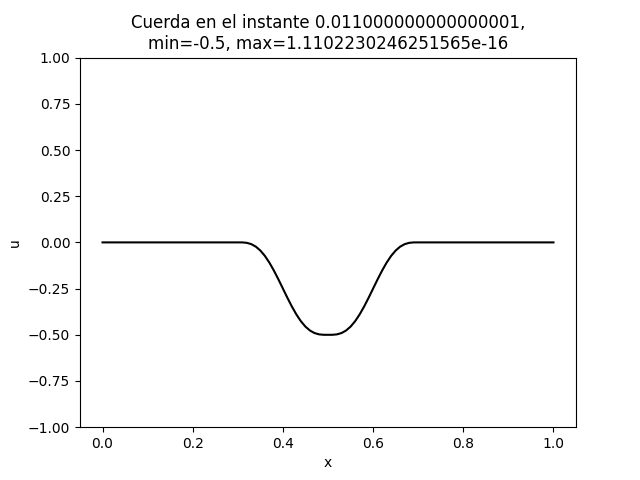
\includegraphics[scale=0.45]{Ejemplo1.png}
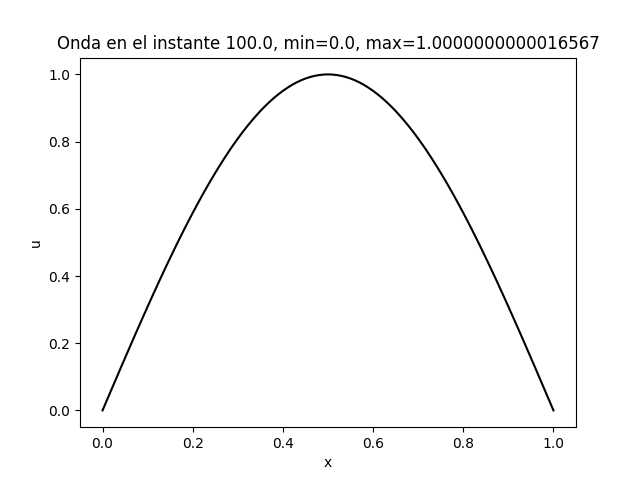
\includegraphics[scale=0.45]{Ejemplo2.png}\\

Supongamos que la cuerda no est� en reposo, habr� una fuerza tensora $T$, producidas por los puntos en los que est� sujeta. Nos apoyaremos en la siguiente figura para ver como se describir�a la ecuaci�n: 
\newpage

\begin{figure}[!ht]
	\centering
	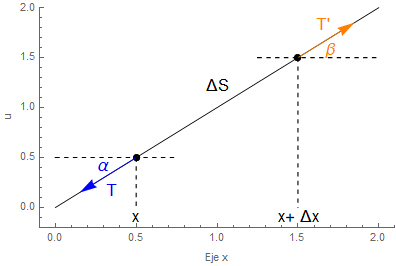
\includegraphics[scale=0.45]{modelado.png}
	\caption{Representaci�n de una secci�n diferencial de la cuerda y las fuerzas asociadas a la misma.}
\end{figure}

Elegido un segmento diferencial del arco de la cuerda $\Delta S$, nos damos cuenta de que la cuerda se habr� desplazado perpendicularmente una cantidad $u$. Por lo tanto la fuerza tensora que produce cada punto en el que est� fijado, no tendr�n la misma direcci�n y sentido opuesto, sino que tendr�n componente vertical.  Las componentes verticales son:

$$T_y= -\mathbb{F_T}sen(\alpha), $$
$$T'_y= F_Tsen(\beta).$$

Luego la fuerza vertical quedar�a $F=F_T(sen(\beta)-sen(\alpha))$, donde $F_T$ es la fuerza generada por la tensi�n, por otro lado, al encontrarnos en una secci�n diferencial los �ngulos son tan peque�os que podemos decir $sen(\alpha) \approxeq tan(\alpha)$ y $sen(\beta) \approxeq tan(\beta)$ quedando

$$F=F_T(tan(\beta)-tan(\alpha)).$$

Adem�s $tan(\alpha)$ y $tan(\beta)$ son las pendientes de la curva en los puntos $x$ y $x+\Delta x$ respectivamente, entonces podemos expresarlos como la primera derivada en los puntos correspondientes $tan(\alpha)=u_x(x,t)$ y $tan(\beta)=u_x(x+\Delta x,t)$. Obtenemos $F=F_T(u_x(x+\Delta x,t)-u_x(x,t))$.\\

Aplicando ahora la segunda Ley de Newton, la fuerza debe ser la masa por la aceleraci�n. Luego ser� la masa $\rho_l \Delta S$, donde $\rho_l $ es la densidad lineal de masa de la cuerda y como estamos en un ambiente diferencial podemos aproximar $\Delta S \approxeq \Delta x $, y la aceleraci�n $u_{tt}(x,t)$. Reestructurando la ecuaci�n queda:

$$u_{tt}(x,t)=\frac{F_T}{\rho_l}\frac{u_x(x+\Delta x,t)-u_x(x,t)}{\Delta x}.$$

Tomando limite cuando $\Delta x\rightarrow 0$ y $c^2=\frac{F_T}{\rho_l}$ la ecuaci�n queda de la siguiente forma:
\begin{equation}\label{eq:basica}
	u_{tt}=c^2u_{xx},\quad (0,l) \times[0,T).
\end{equation}

En este caso podemos tomamos el dominio como $\Omega^1\subset \mathbb{R}$, donde $T$ es un par�metro dado que representa el instante final de la observaci�n. A�adiendo las condiciones de frontera y contorno mas usadas, para m�s informaci�n sobre el tema \citep{Ganzha}, nuestro esquema nos queda. 

\begin{equation}\label{ecuaciononda}
	\begin{array}{lc}   
		u_{tt}-c^2u_{xx}=0, & (x,t)\in (0,L)\times(0,T),
	\end{array}
\end{equation} 
\begin{equation}\label{eq:frontera1}
	\begin{array}{lc}   
		u(x,0)=f(x), &   x\in (0,L),
	\end{array}
\end{equation} 
\begin{equation}\label{eq:frontera2}
	\begin{array}{lc}   
		u_t(x,0)=g(x), &  x \in(0,L),
	\end{array}
\end{equation} 
\begin{equation}\label{eq:frontera3}
	\begin{array}{lc}   
		u(0,t)=u(l,t)=0, &  t\in(0,T).
	\end{array}
\end{equation} 

 Estas �ltima condici�n, \eqref{eq:frontera3}, se llaman de tipo Dirichlet homogenea.




\section{Clasificaci�n de la ecuaci�n de onda}
En esta secci�n clasificaremos la EDP, estas se clasifican en: el�pticas, hiperb�licas y parab�licas. Para poder realizar la clasificaci�n primero tendremos que estandarizarla. Aunque las ecuaciones se pueden clasificar y estandarizar siempre, nosotros por simplicidad lo haremos solo para las de segundo orden.

Una ecuaci�n de segundo orden en forma est�ndar ser�a como sigue:
\begin{equation}\label{eq:estandarizacion}
	Au_{tt}+Bu_{tx}+Cu_{xx}+Du_{t}+Eu_{x}+Fu= G,
\end{equation}
donde $A,B,C,D,E,F,G$ son funciones de variables x y t.\\
Clasificaremos \eqref{eq:estandarizacion} dependiendo de  las ecuaciones caracter�sticas relativas a la ecuaci�n en derivadas parciales (EDP):

\begin{definicion}[label={clasificacion},nameref={Title or anything else}]{Clasificaci�n de las EDP de segundo orden}	
	
	Si en todos los puntos $(x,t)$ de una regi�n $W\subset \mathbb{R}^2$ se cumple que:
	\begin{itemize}
		\item $B^2(x,t)-4A(x,t)C(x,t)>0$, entonces la EDP \eqref{eq:estandarizacion} se dice hiperb�lica.
		\item $B^2(x,t)-4A(x,t)C(x,t)=0$, entonces la EDP \eqref{eq:estandarizacion} se dice parab�lica.
		\item $B^2(x,t)-4A(x,t)C(x,t)<0$, entonces la EDP \eqref{eq:estandarizacion} se dice el�ptica.
		
	\end{itemize}
\end{definicion}

Vemos que siguiendo la notaci�n de  \eqref{eq:basica}, $A=1, C=-c^2, G=f$ y cada una de las dem�s funciones es 0. Ahora tenemos $B^2-4AC=4c^2>0$ y por lo tanto nuestra ecuaci�n es hiperb�lica.\\
Este tipo de clasificaci�n de las ecuaciones la usaremos para separar los distinto m�todos num�ricos que se pueden usar, ya que estos suelen diferir dependiendo de la misma.





\section{Soluciones de tipo onda viajera}
\label{sec:Ecuaciontransporte}
Una vez definida nuestra ecuaci�n de onda, es interesante ver que esta admite dos soluciones de tipo onda viajera uno de los dos sentidos del eje $X$. Para ello comenzaremos suponiendo que la soluci�n $u(x,t)$ se puede descomponer en dos funciones de propagaci�n, donde $c$ sabemos que es la velocidad de la onda,

\begin{equation}\label{eq:propagacion}
	u(x,t)=p_+(x-ct)+p_-(x+ct),
\end{equation}
aqu� llamamos $p_+$ a la propagaci�n hacia la derecha y $p_-$ hacia la izquierda. Ahora siguiendo \citep{strauss}, veamos como ser�a la resoluci�n del problema de valores iniciales, \eqref{ecuaciononda} a \eqref{eq:frontera3} teniendo en cuenta \eqref{eq:propagacion}. Para ello necesitaremos suponer la derivabilidad de $f$.\\

Comenzamos utilizando \eqref{eq:frontera1}, para $t=0$ tendremos,

\begin{equation}\label{eq:fsustituidop}
	f(x)=u(x,0)=p_+(x)+p_-(x),
\end{equation}
derivando \eqref{eq:fsustituidop} en $x$,
\begin{equation}\label{eq:fderivadop}
	f'(x)=p_{+\ x}(x)+p_{-\ x}(x).
\end{equation}

Ahora queremos sustituir el valor de $u_t(x,0)$ en la condici�n \eqref{eq:frontera2}, para ello derivemos antes \eqref{eq:propagacion} respecto a $t$,

\begin{equation}\label{eq:derivadasp}
	u_t=\frac{\partial}{\partial t}(p_+(x-ct)+p_-(x-ct))=cp_+'(x+ct)-cp_-'(x-ct),
\end{equation}
entonces,
\begin{equation}\label{eq:gsustituidop}
	g(x)=u_t(x,0)=-cp_+(x)+cp_-(x),
\end{equation}
dividiendo la igualdad por $c$,

\begin{equation}\label{eq:gderivadop}
	\frac{1}{c}g(x)=-p_+(x)+p_-(x).
\end{equation}

Haciendo \eqref{eq:fsustituidop} $+$  \eqref{eq:gsustituidop} y \eqref{eq:fsustituidop} $-$  \eqref{eq:gsustituidop}:

$$f'(x) + \frac{1}{c}g(x)= 2p_-'(x),\quad \textbf{y}\quad f'(x) - \frac{1}{c}g(x)= 2p_+'(x).$$

Luego despejando, 

$$p_-'(x)= \frac{1}{2}f'(x) + \frac{1}{2c}g(x),\quad \textbf{y}\quad p_+'(x)= \frac{1}{2}f'(x) - \frac{1}{2c}g(x).$$

Como todo este proceso podr�a hacerse para todo $x\in \mathbb{R}$, integrando respecto a $x$ y sustituy�ndolo por $x+ct$ y $x-ct$, respectivamente, obtendremos las representaciones siguientes de $p_-$ y $p_+$.
\begin{equation}\label{repp-}
	p_-(x+ct)=\frac{1}{2}f(x+ct) + \frac{1}{2c}\int_{0}^{x+ct}g(s)\partial s +A,
\end{equation}
\begin{equation}\label{repp+}
	p_+(x+ct)=\frac{1}{2}f(x-ct) - \frac{1}{2c}\int_{0}^{x-ct}g(s)\partial s +B,
\end{equation}
donde $A,B$ son constantes que tomaremos como 0 al saber que $A+B=$ gracias a \ref{eq:propagacion}. Nuestras integrales comienzan en $0$ por el dominio de \ref{ecuaciononda}.\\

Finalmente llegamos. a que  la soluci�n del problema de valores iniciales, ser�:
\begin{equation*}
	u(x,t)= \frac{1}{2}\left(f'(x+ct)+f'(x-ct)\right) + \frac{1}{2c}\int_{x-ct}^{x+ct}g(s)\partial s. 
\end{equation*}



\section{La energ�a en la ecuaci�n de onda}
\label{sec:energiaondas}

En esta secci�n nos centraremos en analizar la ley de energ�a en la ecuaci�n de onda. Llamemos $S=(0,L)$. Para poder obtener el la energ�a de la ecuaci�n haremos el producto interior \ref{Inner} de la misma con $u_t$:

\begin{equation*}
	\left<u_t(\cdot,t),u_{tt}(\cdot,t)\right>_S = c^2\left<u_{t}(\cdot,t),u_{xx}(\cdot,t)\right>_S.
\end{equation*} 

Para facilitar el entendimiento de la secci�n simplificaremos la notaci�n de la siguiente forma:
\begin{equation}\label{ondaut}
	\left<u_t,u_{tt}\right>_S = c^2\left<u_{t},u_{xx}\right>_S.
\end{equation} 

Sabiendo que siempre estaremos fijando el instante t. Cada uno de los t�rminos de la energ�a tendremos que ponerlo de la forma $\frac{\partial}{\partial t}\left(\cdot\right)$, comenzaremos por el termino de la izquierda. Para desarrollarlo necesitaremos la siguiente igualdad, derivada de la integraci�n por partes,

\begin{equation}\label{eq:intpartes}
	\left<u_{t},u_{tt}\right>_S= \int_S u_tu_{tt} \partial x = \left.u_tu_t\right|_S- \int_S u_{tt}u_{t} \partial x = \left.u_tu_t\right|_S- \left<u_{tt},u_{t}\right>_S .
\end{equation}

Por otro lado necesitaremos ver como se puede descomponer $\frac{\partial}{\partial t}||u_t||_S^2$, utilizando la definici�n de norma \ref{Inner},

\begin{equation*}
	\frac{\partial}{\partial t}||u_t||_S^2 = \frac{\partial}{\partial t}\int_S u_tu_t \partial x. 
\end{equation*}

Ya que, $\frac{\partial}{\partial t}$ independiente de $x$, y suponiendo que se dan en $u$ y en $u_t$ condiciones de continuidad adecuadas, podremos permutar de sitio la integral y la derivada, y por tanto,
\begin{equation*}
	\frac{\partial}{\partial t}||u_t||_S^2 = \int_S \frac{\partial}{\partial t} u_t u_t \partial x, 
\end{equation*}
derivando, usando la regla de la cadena, y separando en dos integrales obtenemos la igualdad

\begin{equation}\label{eq:normau}
	\begin{split}
		\frac{\partial}{\partial t}||u_t||_S^2 &= \int_S u_{tt} u_{t}+u_{t} u_{tt} \partial x\\
		&=\int_S u_{tt} u_{t}\partial x +\int_S u_{t} u_{tt} \partial x\\
		&=\left<u_{tt},u_{t}\right>_S+\left<u_{t},u_{tt}\right>_S.
	\end{split}
\end{equation}

Continuando ahora desde nuestro factor inicial $\left<u_{t},u_{tt}\right>_S$, usando la igualdad \eqref{eq:normau},

\begin{equation*}
	\left<u_{t},u_{tt}\right>_S=\int_S u_{t}u_{tt}\partial x=\frac{\partial}{\partial t}||u_t||_S^2 -\int_S u_{tt}u_{t}\partial x.
\end{equation*}

Utilizando \eqref{eq:intpartes} en el �ltimo sumando,

\begin{equation*}
	\left<u_{t},u_{tt}\right>_S=\frac{\partial}{\partial t}||u_t||_S^2 -\left(\left.u_tu_t\right|_S-\int_S u_{t}u_{tt}\partial x  \right).
\end{equation*}

Agrupando los t�rminos tendremos,
\begin{equation*}
	2\left<u_{t},u_{tt}\right>_S= \frac{\partial}{\partial t}||u_t||_S^2 - \left.u_tu_t\right|_S,
\end{equation*}
\begin{equation}\label{eq:primerfactor}
	\left<u_{t},u_{tt}\right>_S=\frac{1}{2} \frac{\partial}{\partial t}||u_t||_S^2 -\frac{1}{2} \left.u_tu_t\right|_S.
\end{equation}



Ahora nos centraremos en el termino de la derecha, comenzamos utilizando la igualdad \eqref{eq:intpartes}, y pasamos el producto interior hacia la izquierda en \eqref{ondaut}, quedando,
\begin{equation}\label{ondau_t2}
	\left<u_t,u_{tt}\right>_S  -c^2\left<u_{tx},u_{x}\right>_S = \left.u_tu_x\right|_S
\end{equation} 

Siguiendo con el an�lisis de  $\left<u_{tx},u_{x}\right>_S$, an�logamente a como lo hicimos con $\left<u_t,u_{tt}\right>_S$, obtendremos 

\begin{equation}\label{eq:segundofactor}
	\left<u_{tx},u_{x}\right>_S=\frac{1}{2}\frac{\partial}{\partial t}\int_{\mathbb{R}}u_{x}u_{x} \partial x -\frac{1}{2} \left.u_xu_x\right|_S=\frac{1}{2} \frac{\partial }{\partial t}||u_{x}||^2 -\frac{1}{2} \left.u_xu_x\right|_S.
\end{equation}

Introduciendo \eqref{eq:primerfactor} y \eqref{eq:segundofactor} en la ecuaci�n \eqref{ondau_t2} queda:

$$\frac{\partial}{\partial t}\left( \frac{1}{2}||u_t||^2+\frac{c^2}{2}||u_x||^2\right)= c^2\left.u_tu_x\right|_S-\frac{c^2}{2} \left.u_xu_x\right|_S -\frac{1}{2} \left.u_tu_t\right|_S .$$


Definiremos $\mathfrak{B}\triangleq  c^2\left.u_tu_x\right|_S+\frac{c^2}{2} \left.u_xu_x\right|_S +\frac{1}{2} \left.u_tu_t\right|_S $.\\
Ahora podremos separar en energ�a cin�tica $K= \frac{1}{2}||u_t||^2$ y la energ�a potencial $P = \frac{c^2}{2}||u_x||^2 $ de donde se sigue que la energ�a total ser�
$$\mathfrak{H}= K+ P= \frac{1}{2}||u_t||^2 +\frac{\mu^2}{2}||u_x||^2 .$$

Por otro lado, tenemos que $\frac{\partial}{\partial t}\mathfrak{H}=\mathfrak{B}$, para que se diese conservaci�n de la energ�a tendr� que ser $\mathfrak{B}=0$. Desarrollandolo,

\begin{equation*}
	\begin{split}
		0=\mathfrak{B}&=c^2(u_t(l,t)u_x(l,t)-u_t(0,t)u_x(0,t))+\frac{c^2}{2} \left(u_x(l,t)u_x(l,t)-u_x(0,t)u_x(0,t)\right)\\
		& +\frac{1}{2} \left(u_t(l,t)u_t(l,t)-u_t(0,t)u_t(0,t)\right).
	\end{split}
\end{equation*}


Vemos que esto nos impone ciertas restricciones a nuestra ecuaci�n, estas se traducir�n a condiciones de contorno en nuestro esquema.




% ----------------------------------------------------------------------



	
% Comienza ahora con el trabajo en sí y divídelo en las partes que consideres para su mejor comprensión.
% !TeX encoding = ISO-8859-1
\chapter{EXPERIMENTOS COMPUTACIONALES}
\label{cha:arbolesclasificacion}

En esta secci�n se analizar�n los m�todos explicados en la Secci�n \ref{cha:svmmulticlase} estos son, OVO, OVA, DAGSVM, Modelo Weston-Watkins y Modelo Crammer-Singer, el objetivo es comparar los resultados obtenidos al aplicar dichos m�todos. Los experimentos que se llevar�n a cabo en esta secci�n han sido realizado en el entorno Jupyter usando el lenguaje de programaci�n Python. \\

Para los modelos OVO, OVA y Crammer-Singer se han utilizado librer�as del paquete sklearn que los resuelven mientras que por otro lado para los modelos DAGSVM y Weston-Watkins se ha tenido que desarrollar el c�digo para resolverlos, puesto que no existen librer�as como en los casos anteriores que los resuelvan.


\section{CONJUNTOS DE ENTRENAMIENTO}

Para realizar los experimentos computacionales se han usado 3 bases de datos las cuales se pueden encontrar en el repositorio UCI, estas bases de datos contienen una peque�a cantidad de atributos debido al incremento en tiempo computacional que supondr�a hacer los c�lculos con m�s atributos. A continuaci�n se explicar� brevemente las bases de datos que se utilizar�n.\\

\begin{itemize}
	\item IRIS: Es una de las bases m�s usadas en reconocimiento de patrones. Esta base de datos posee 150 plantas de g�nero Iris, en concreto a lo largo de las 150 observaciones nos encontramos con 3 clases distintas, Iris Setosa, Iris Versicolour e Iris Virginica, cada una de ellas con 50 de las 150 observaciones de la base de datos. Posee 4 atributos que son longitud y anchura del s�palo y del p�talo.  
	\item Contraceptive Method Choice (CMC): En este base de datos se posee informaci�n de 1473 mujeres casadas, en concreto se han estudiado 10 caracter�sticas de estas mujeres como la edad, n� de hijos que ha tenido, su educaci�n, la educaci�n de su pareja... La variable que determina la clase es que m�todo anticonceptivo usan, existen tres posibilidades, que no usen, un m�todo de larga duraci�n o un m�todo de corta duraci�n.
	\item Car Evolution Database (CED): Esta base de datos dispone de informaci�n sobre 1728 coches, en concreto el estudio provee 6 atributos para cada coche como n�mero de puertas, precio de compra, capacidad del veh�culo..., y as� clasifica los coches en 4 clases diferentes. %https://archive.ics.uci.edu/ml/datasets/Car+Evaluation
\end{itemize}
	%Wine (W): Esta base de datos dispone de informaci�n sobre 178 an�lisis a vinos que han crecido en la misma zona de Italia, pero provienen de 3 cultivos diferentes. Como resultado de cada an�lisis conocemos 13 atributos de cada vino que se ha estudiado.

La tabla de abajo muestra un peque�o resumen de las propiedades que conocemos de las bases de datos, la variable \textbf{m} corresponde con el n�mero de datos, \textbf{d} con la cantidad de atributos y \textbf{n} el n�mero de clases.

\begin{table}[H]
	\begin{center}
		\begin{tabular}{ | m{2.5cm} | m{2.5cm} | m{2.5cm} | m{2.5cm} | }
			\hline {\centering}Bases de datos &  \centering \textbf{m} & \centering \textbf{d} & \hspace{11mm}\textbf{n} \\ \hline
		    \centering IRIS & \centering$150$ & \centering $4$ &\hspace{10mm}  3 \\ \hline
			\centering CMC &\centering $1473$ & \centering $10$ &\hspace{10mm}  3 \\ \hline
			\centering CED & \centering{$1728$}&\centering $6$  &\hspace{10mm}  4 \\ \hline
		\end{tabular}
	\end{center}
\end{table}

\section{RESULTADOS PREVIOS}
\textbf{COMENTARIO: Quiero escribir la tarjeta que estoy usando para hacer las operaciones en python.}.\\

Para valorar la eficiencia de cada m�todo, se utilizar�n los valores de ACC, el par�metro C que da mayor precisi�n a cada m�todo y el tiempo que tarda el programa en realizar el entrenamiento del modelo y la obtenci�n de estos valores. A continuaci�n explicaremos con m�s detalle los dos primeros valores que se han expuesto.
\begin{itemize}
	%\item AUC: Este indicador se puede interpretar como la probabilidad  de que el clasificador pueda distinguir entre las diferentes clases. Su f�rmula es la siguiente 
	%\begin{equation}\nonumber
	%AUC =\frac{\frac{VP}{VP+FN}+\frac{VN}{VN+FP}}{2}
	%\end{equation}
	\item ACC: Este valor nos indica la calidad del modelo, esto es, el porcentaje de elementos clasificados correctamente. 
	\begin{equation}\nonumber
	ACC =\frac{VP+VN}{VP+VN+FP+FN}
	\end{equation} 
	siendo VP,VN,FP y FNv denonimados como verdaderos positivos, verdaderos negativos, falsos positivos y falsos negativos respectivamente y corresponden a los valores que se encuentran en la matriz de confusi�n.\\
	
	%esta p�gina para tablas y tal est� to bien https://www.ucm.es/data/cont/docs/1346-2019-04-12-BaSix%20LaTeX%20ba%CC%81sico%20con%20ejercicios%20resueltos%20-%20Noir16.pdf
	
	
	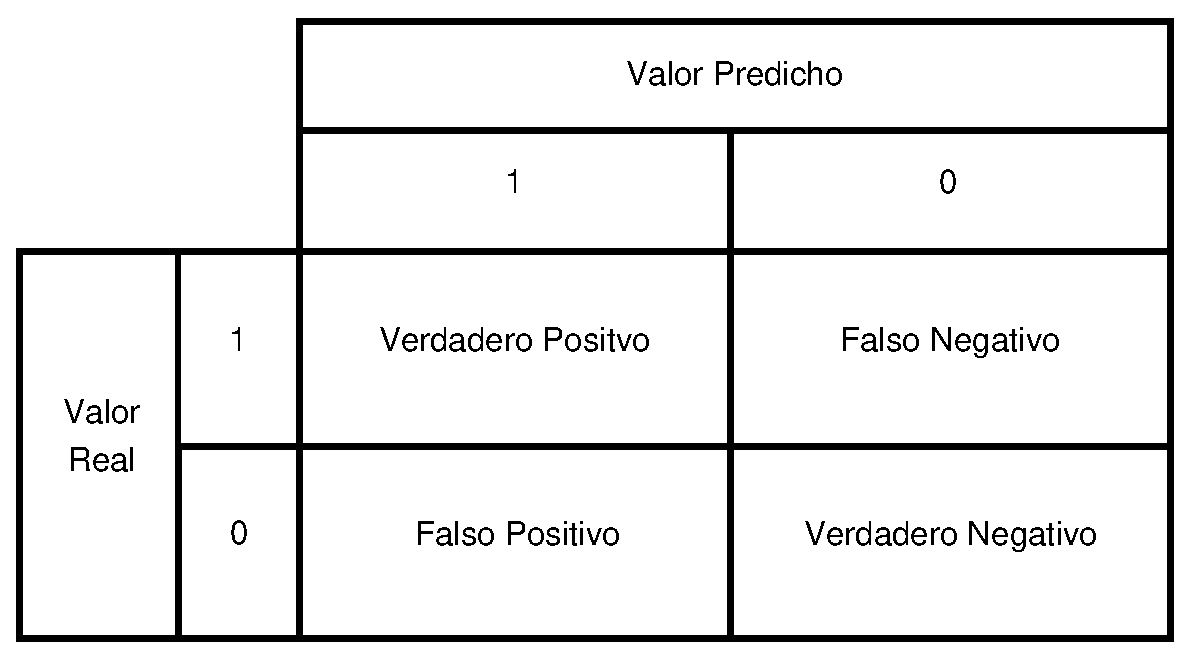
\includegraphics[width=0.8\textwidth]{matrizconfusion.eps}
	\item Par�metro C: Con este par�metros se penaliza el uso de las variable de holgura $\boldsymbol{\xi}$. Para la obtenci�n del par�metro C utilizaremos la t�cnica de la validaci�n cruzada (Cross Validation), para este proceso se busca dividir los datos en T pliegues o conjuntos, de estos T pliegues se utilizan (T-1) para el entrenamiento del modelo y el restante para la fase de testeo, el algoritmo en cuesti�n se entrenar� y probar� T veces, cada vez que se utiliza un nuevo conjunto como conjunto de prueba. Los par�metros que se probar�n de C son los siguientes $$C=\{2^{-4},2^{-3},2^{2},2^{-1},1,2,2^{2},2^{3},2^{4}\}$$ \\
	
\end{itemize}

\textbf{COMENTARIO: Tengo que a�adir las tablas con los resultados, pero estoy programando los m�todos DAGSVM y WW, que no vienen en librer�as de python, y la divisi�n en grupos de 5 con una proporci�n de clases parecida en cada grupo.}

%https://www.iartificial.net/precision-recall-f1-accuracy-en-clasificacion/  \quad (HAY OTRA PAGINA ESCRITA EN COMENTARIO, PORQUE ME DA UN ERROR AL ESCRIBIRLA TAL CUAL)\\
%https://sitiobigdata.com/2019/01/19/machine-learning-metrica-clasificacion-parte-3/# 
%ACCURACY: 	porcentaje total de elementos clasificados correctamente. $$\frac{TP+TN}{TP+TN+FP+FN}$$
%Es un valor entre 0 y 1. Cuanto m�s alto, mejor. No funciona bien cuando las clases est�n desbalanceadas, pero creo que yo si lo voy a balancear.\\
%RECALL/TASA DE A TP/SENSIBILIDAD: Es el n�mero de elementos identificados correctamente como positivos del total de positivos verdaderos.$$\frac{TP}{TP+FN}$$\\
%PRECISION: n�mero de elementos identificados correctamente como positivo de un total de elementos identificados como positivos $$\frac{TP}{TP+FP}$$\\

%Precisi�n trata de ser preciso. Entonces, incluso si logramos capturar solo un caso de c�ncer y lo capturamos correctamente, entonces somos 100\% precisos.\\

%Recall no se trata tanto de capturar casos correctamente sino m�s de capturar todos los casos que tener ?c�ncer? con la respuesta como ?c�ncer?. Entonces,
%si siempre decimos cada caso como ?c�ncer?, tenemos un recuerdo del 100\%.\\

%Entonces, b�sicamente, si queremos enfocarnos m�s en minimizar los falsos negativos, deseamos que nuestro recuerdo sea lo m�s cercano posible al 100\% sin la precisi�n es muy mala y si queremos enfocarnos en minimizar los falsos positivos, entonces nuestro enfoque debe orientarse a hacer que la Precisi�n sea lo m�s cercana posible al 100\%.\\
%EXACTITUD\\

%AUC\\


%�RBOLES DE CLASIFICACI�N

%Si la entrop�a es 0, entonces es no se sigue m�s por ese lado. Si la entrop�a es 1 entonces los datos est�n divididos equitativamente.\\

%Information gain (ganancia de informaci�n) el resultado es la caracter�stica con mejores resultados para separar los datos. A menores valores de entrop�a, mayor informaci�n se gana, y por el contrario a mayor valor de entrop�a menor informaci�n.\\

%El algoritmo ID3 est� relacionado con la ganancia de informaci�n???. Osea creo que todo lo que veo es el algoritmo ID3.\\

%Un valor se puede parar, porque todos los nodos tengan entrop�a 0, porque se imponga una profunidad al �rbol o porque se llegue a un n�mero menor de valores deseados (no se si hay m�s posibilidades).\\

%La diferencia entre entrop�a y gini impurity es que en el primero se alcanza el m�ximo en 1 y en el segundo en 0.5, pero creo que el concepto en ambos es el mismo. Gini impurity es m�s sencillo de resolver, porque con la entrop�a tiene un log y el otro solo tiene un cuadrado.\\

% ----------------------------------------------------------------------

	

% !TeX encoding = ISO-8859-1

\chapter{Modelado en Python y comparativa}
\label{cha:Comparativa}

En este cap�tulo nos centraremos en ver el modelado en Python de nuestro esquema resuelto por el m�todo de diferencias finitas, \eqref{esquemacompletoonda}. Veremos como var�a la soluci�n en varios instantes de tiempo, la forma que presenta la onda cambiando las condiciones iniciales \eqref{eq:esquemafrontera1} y \eqref{eq:esquemafrontera2}, y haremos una comparativa de como afectan las condiciones de estabilidad \eqref{mu}, y de conservaci�n de la energ�a \eqref{energiacero}.

\section{Soluciones}
\label{sec:soluciones}
En esta secci�n comenzaremos se�alando varias soluciones dependiendo de las condiciones iniciales. En toda la secci�n establecemos $c=440$.


\subsection{$f(x)= sin(\pi x)$, $g(x)=0$}
\label{subsec:sin(x)}
Cuando la posici�n inicial depende del seno y la velocidad inicial es $0$, se puede observar como nuestra soluci�n oscila sin llegar a parar, al no tener en cuenta nuestro sistema \eqref{esquemacompletoonda}, fuerzas externas como el rozamiento. 

\newpage
	
\begin{figure}[ht]
	\centering
	\begin{minipage}[b]{0.45\textwidth}
		\centering
		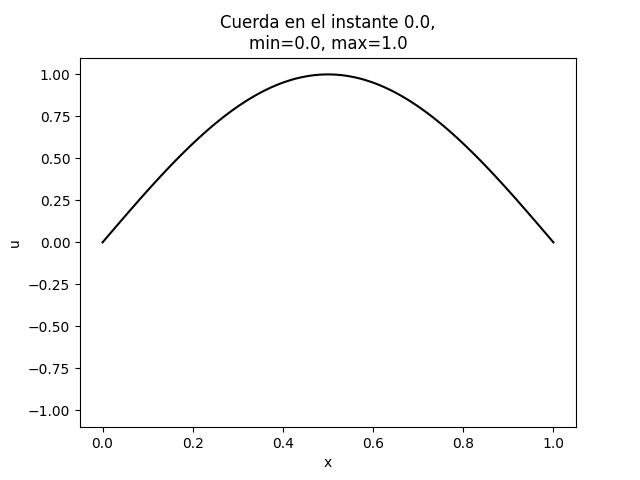
\includegraphics[width=\textwidth]{Seno1.png}
		\caption{Posici�n inicial de la cuerda.}
		\label{fig:Seno1}
	\end{minipage}
	\hfill
	\begin{minipage}[b]{0.45\textwidth}
		\centering
		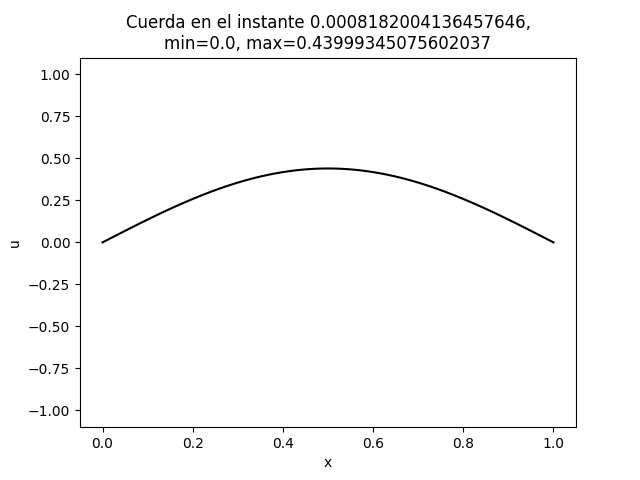
\includegraphics[width=\textwidth]{Seno2.png}
		\caption{La cuerda comienza a bajar.}
		\label{fig:Seno2}
	\end{minipage}
\end{figure}

\begin{figure}[ht]
	\centering
	\begin{minipage}[b]{0.45\textwidth}
		\centering
		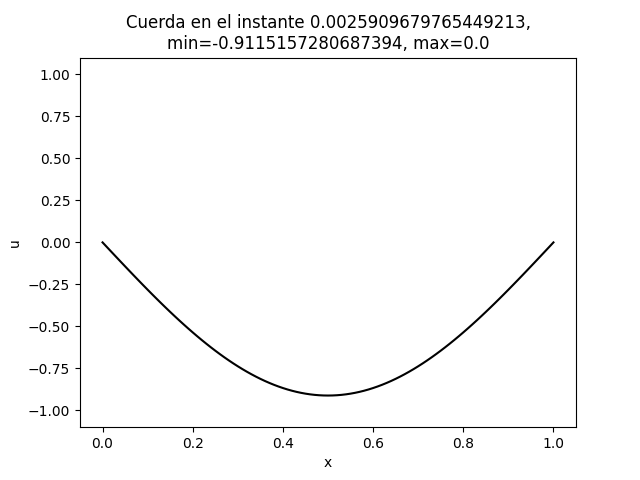
\includegraphics[width=\textwidth]{Seno3.png}
		\caption{Sigue bajando hasta llegar a la posici�n de m�xima amplitud.}
		\label{fig:Seno3}
	\end{minipage}
	\hfill
	\begin{minipage}[b]{0.45\textwidth}
		\centering
		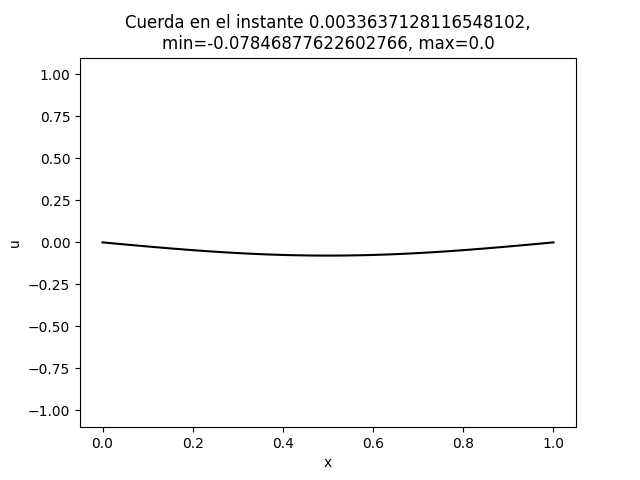
\includegraphics[width=\textwidth]{Seno4.png}
		\caption{La cuerda comienza a subir de nuevo.}
		\label{fig:Seno4}
	\end{minipage}
\end{figure}

\begin{wrapfigure}[4]{r}{0.45\textwidth}
	\vspace{-2cm}
	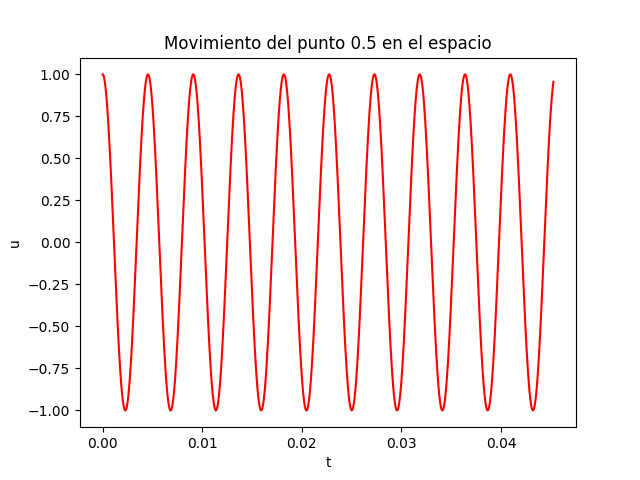
\includegraphics[width=0.45\textwidth]{Seno5.png}
	\caption{Se puede escuchar este sonido en el archivo figura5-5.wav adjunto.}
	\label{fig:Seno5}
	
\end{wrapfigure}

\vspace{2cm}

Este tipo de movimiento es muy regular, podemos observarlo, por ejemplo, en el movimiento del punto el punto $x=0.5$ respecto al tiempo.


\newpage


\subsection{$f(x)$ tipo Struck, $g(x)=0$}
Cuando la posici�n inicial es de tipo Struck, es decir, un pico en la zona central de la cuerda, y la velocidad inicial es $0$, la soluci�n no es tan suave, al ser $f$ no derivable. 

\vspace{2cm}
\begin{figure}[ht]
	\centering
	\begin{minipage}[b]{0.45\textwidth}
		\centering
		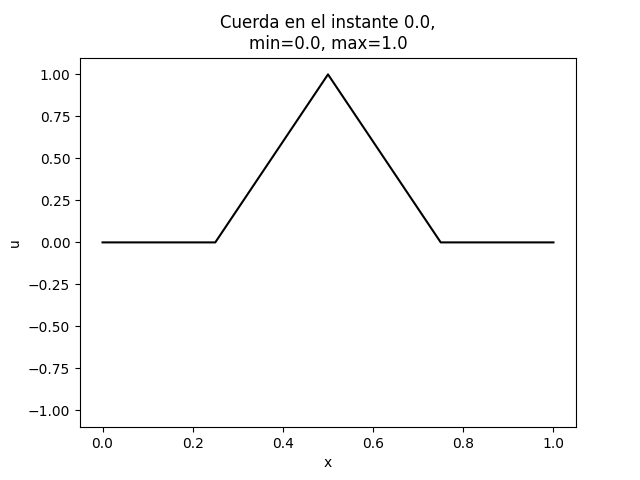
\includegraphics[width=\textwidth]{Pico1.png}
		\caption{Posici�n inicial de la cuerda.}
		\label{fig:Pico1}
	\end{minipage}
	\hfill
	\begin{minipage}[b]{0.45\textwidth}
		\centering
		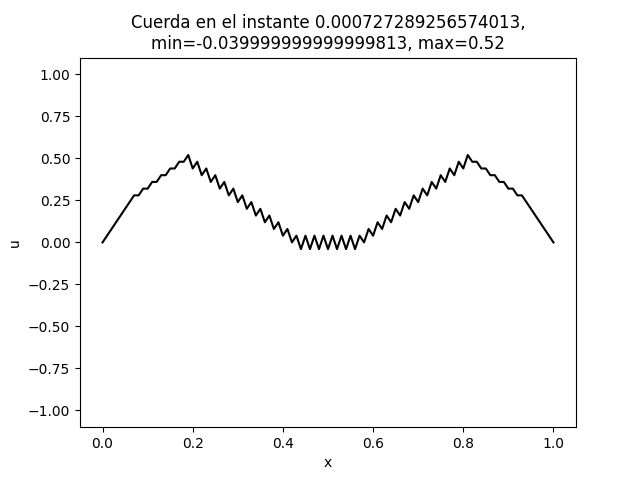
\includegraphics[width=\textwidth]{Pico2.png}
		\caption{Se crean picos en la cuerda.\\}
		\label{fig:Pico2}
	\end{minipage}
\end{figure}
\vspace{1.5cm}
\begin{figure}[ht]
	\centering
	\begin{minipage}[b]{0.45\textwidth}
		\centering
		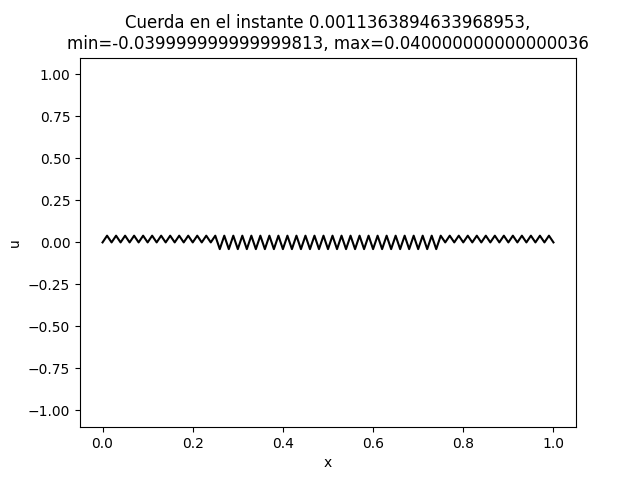
\includegraphics[width=\textwidth]{Pico3.png}
		\caption{}
		\label{fig:Pico3}
	\end{minipage}
	\hfill
	\begin{minipage}[b]{0.45\textwidth}
		\centering
		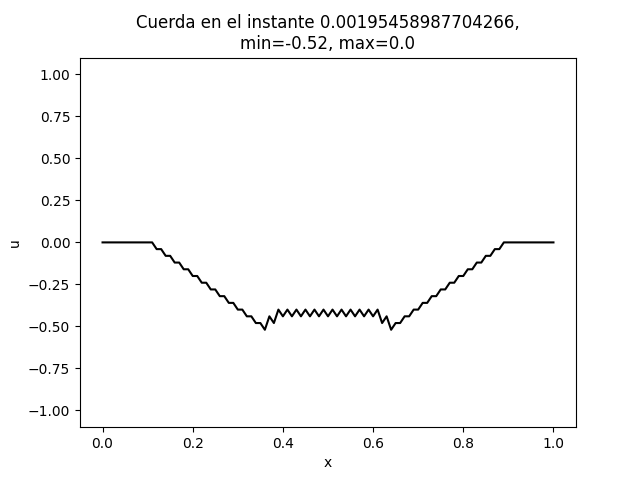
\includegraphics[width=\textwidth]{Pico4.png}
		\caption{}
		\label{fig:Pico4}
	\end{minipage}
\end{figure}
\newpage
En este caso la forma de la onda en cada punto no es tan regular, y cambia mucho dependiendo del punto que observemos, como ejemplo visualizaremos el movimiento de los puntos $x=0.07$  y $x=0.5$.\\
\begin{figure}[ht]
	\centering
	\begin{minipage}[b]{0.45\textwidth}
		\centering
		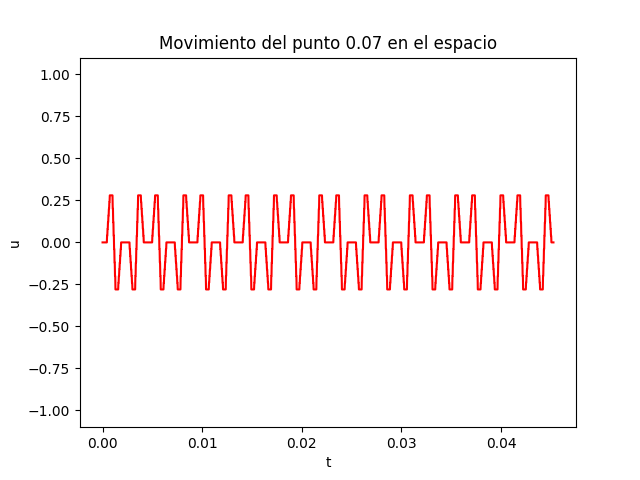
\includegraphics[width=\textwidth]{Pico5.png}
		\caption{Archivo figura5-10.wav}
		\label{fig:Pico5}
	\end{minipage}
	\hfill
	\begin{minipage}[b]{0.45\textwidth}
		\centering
		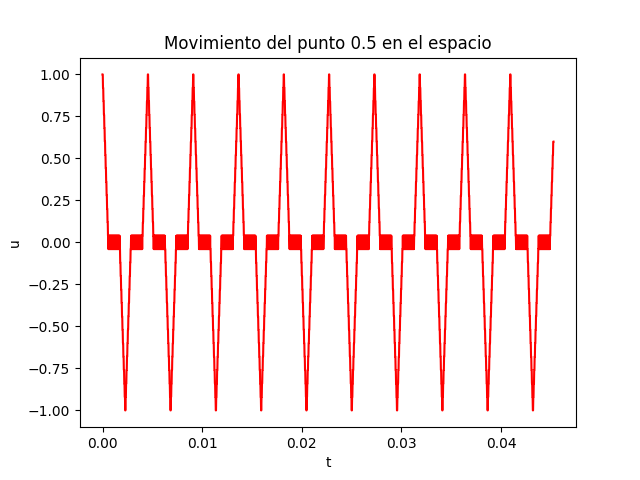
\includegraphics[width=\textwidth]{Pico6.png}
		\caption{Archivo figura5-11.wav}
		\label{fig:Pico6}
	\end{minipage}
\end{figure}

Se observa que la onda var�a dependiendo de la posici�n de la cuerda en las que se haga la observaci�n, por ende, tambi�n el sonido producido.

\subsection{$f(x)= 0$, $g(x)$ tipo Struck}


\begin{wrapfigure}[5]{r}{0.45\textwidth}
	\vspace{-2.2cm}
	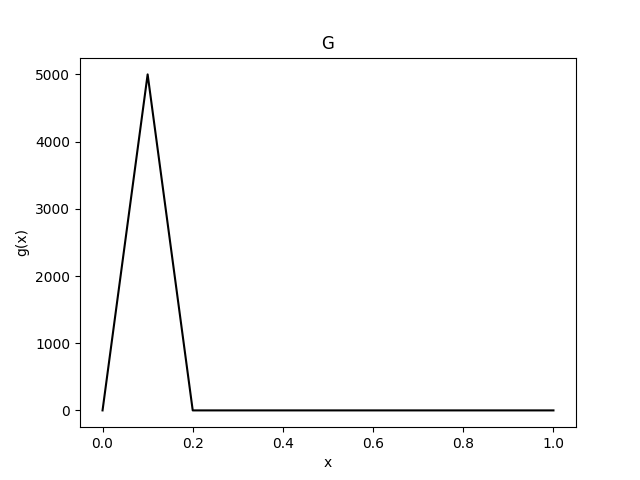
\includegraphics[width=0.45\textwidth]{Planog.png}
	\caption{Velocidad inicial.}
	\label{fig:Planog}
	
\end{wrapfigure}

\vspace{1cm}

En este caso partimos de una onda en reposo, con una velocidad inicial tipo Struck. A la derecha vemos una gr�fica de la forma que tiene esta velocidad inicial.\\ 

\begin{wrapfigure}[4]{r}{0.45\textwidth}
	\vspace{-1.6cm}
	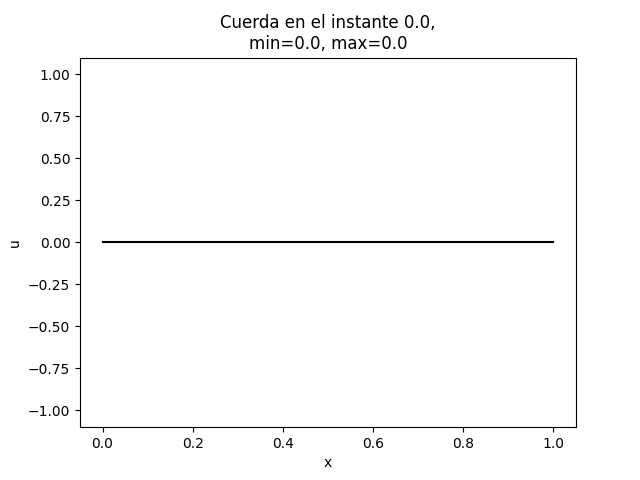
\includegraphics[width=0.45\textwidth]{Plano0.png}
	\caption{Posici�n inicial de la cuerda.}
	\label{fig:Plano0}
	
\end{wrapfigure}
\vspace{1.2cm}
En esta imagen vemos la posici�n inicial. Dependiendo del n�mero de puntos que elijamos en nuestro mallado, podremos ver que la soluci�n se hace m�s suave, lo ilustraremos eligiendo 50 y 200 puntos en el eje espacial.

\newpage
Muestra de la soluci�n con $m=50$.
\begin{figure}[ht]
	\centering
	\begin{minipage}[b]{0.32\textwidth}
		\centering
		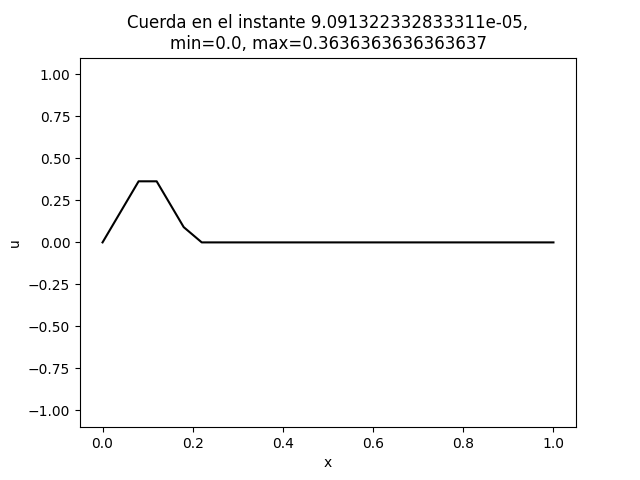
\includegraphics[width=1.1\textwidth]{Plano1.png}
		\caption{}
		\label{fig:Plano1}
	\end{minipage}
	\hfill
	\begin{minipage}[b]{0.32\textwidth}
		\centering
		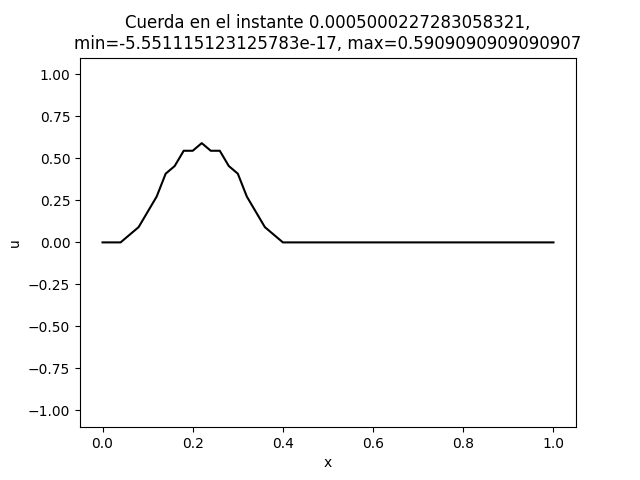
\includegraphics[width=1.1\textwidth]{Plano2.png}
		\caption{}
		\label{fig:Plano2}
	\end{minipage}
	\hfill
	\begin{minipage}[b]{0.32\textwidth}
		\centering
		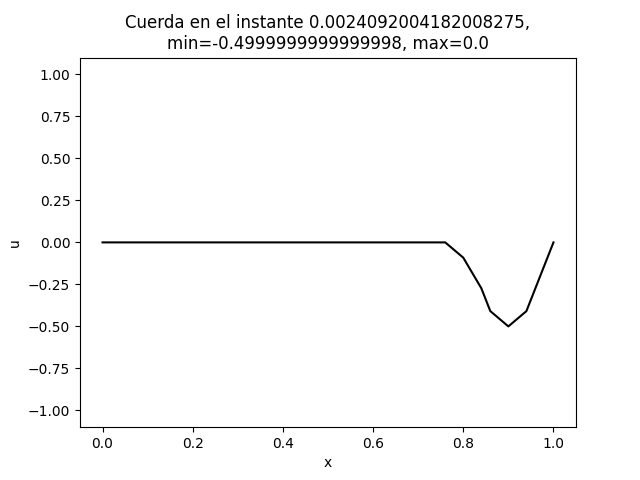
\includegraphics[width=1.1\textwidth]{Plano3.png}
		\caption{}
		\label{fig:Plano3}
	\end{minipage}
\end{figure}

Muestra de la soluci�n con $m=200$:
\begin{figure}[ht]
	\centering
	\begin{minipage}[b]{0.32\textwidth}
		\centering
		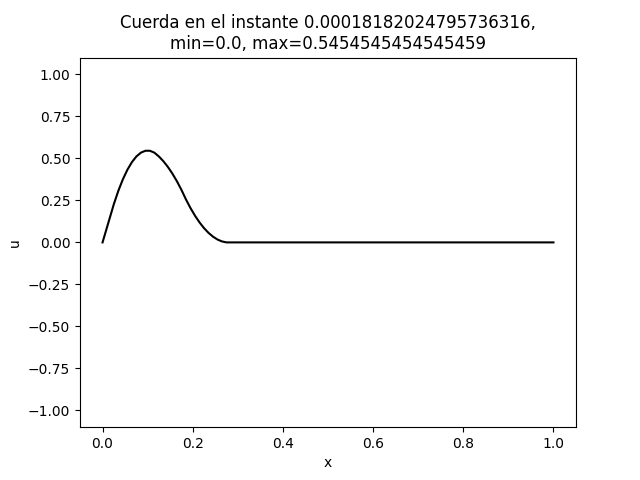
\includegraphics[width=1.1\textwidth]{Plano4.png}
		\caption{}
		\label{fig:Plano4}
	\end{minipage}
	\hfill
	\begin{minipage}[b]{0.32\textwidth}
		\centering
		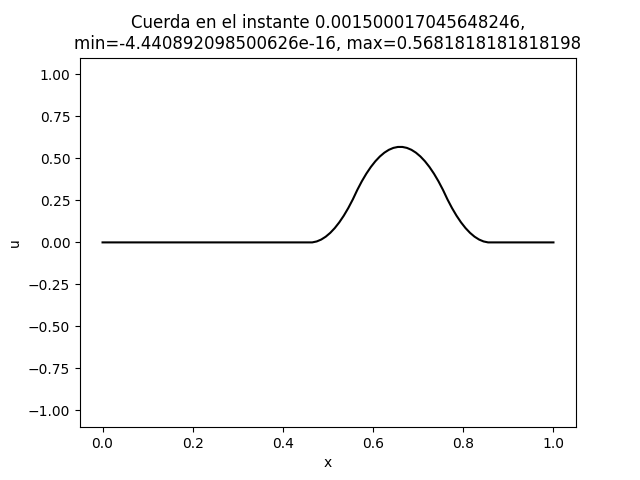
\includegraphics[width=1.1\textwidth]{Plano5.png}
		\caption{}
		\label{fig:Plano5}
	\end{minipage}
	\hfill
	\begin{minipage}[b]{0.32\textwidth}
		\centering
		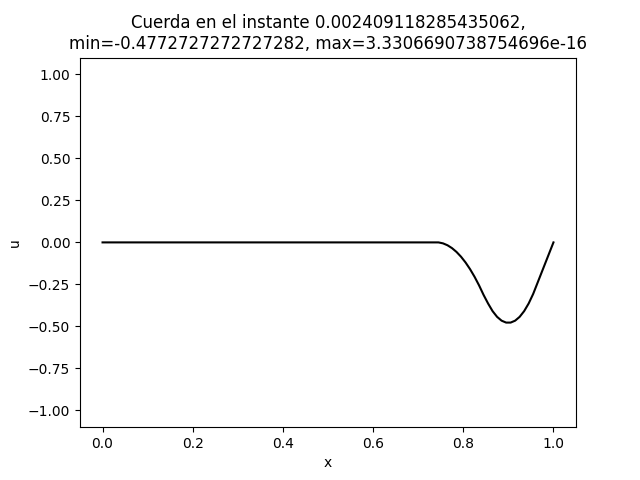
\includegraphics[width=1.1\textwidth]{Plano6.png}
		\caption{}
		\label{fig:Plano6}
	\end{minipage}
\end{figure}

\begin{wrapfigure}[5]{r}{0.45\textwidth}
	\vspace{-1.5cm}
	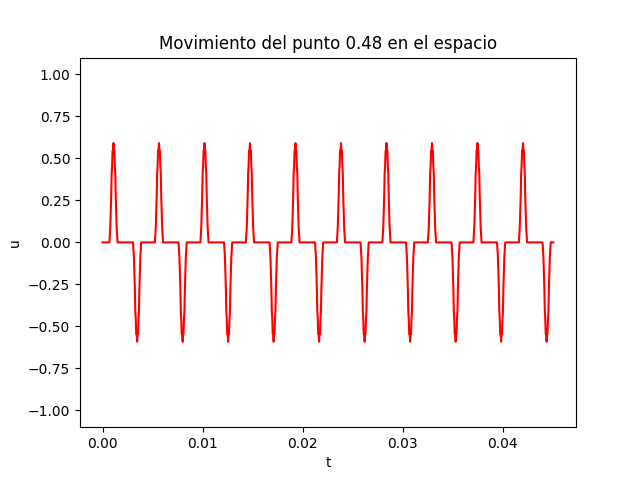
\includegraphics[width=0.45\textwidth]{Planoonda.png}
	\caption{Archivo figura5-20.wav}
	\label{fig:PlanoOnda}
	
\end{wrapfigure}

\vspace{1cm}
A�n as�, para los puntos en los que hacemos la resoluci�n, el movimiento de la onda ser� pr�cticamente id�ntico y la diferencia en el audio indistinguible. Un ejemplo es el esquema de la derecha.\\


\subsection{\textbf{$f(x)= sin(2\pi x)$}, $g(x)=0$}
En cada uno de los casos anteriores, tal y como hemos dicho al principio de la secci�n, $c=440$ y como solo hay dos nodos, puntos en los que la amplitud es siempre $0$, en todos los casos la frecuencia ser� $440Hz$. Esta frecuencia corresponde a un La central (4� octava), la hemos elegido al ser la m�s usual para ejemplificar este tipo de modelado.\\
Ahora, elijamos un caso en el que tengamos $3$ nodos, por ejemplo $f(x)= sen(2\pi x)$, La frecuencia se corresponder� a un La de 5� octava.


\begin{figure}[ht]
	\centering
	\begin{minipage}[b]{0.45\textwidth}
		\centering
		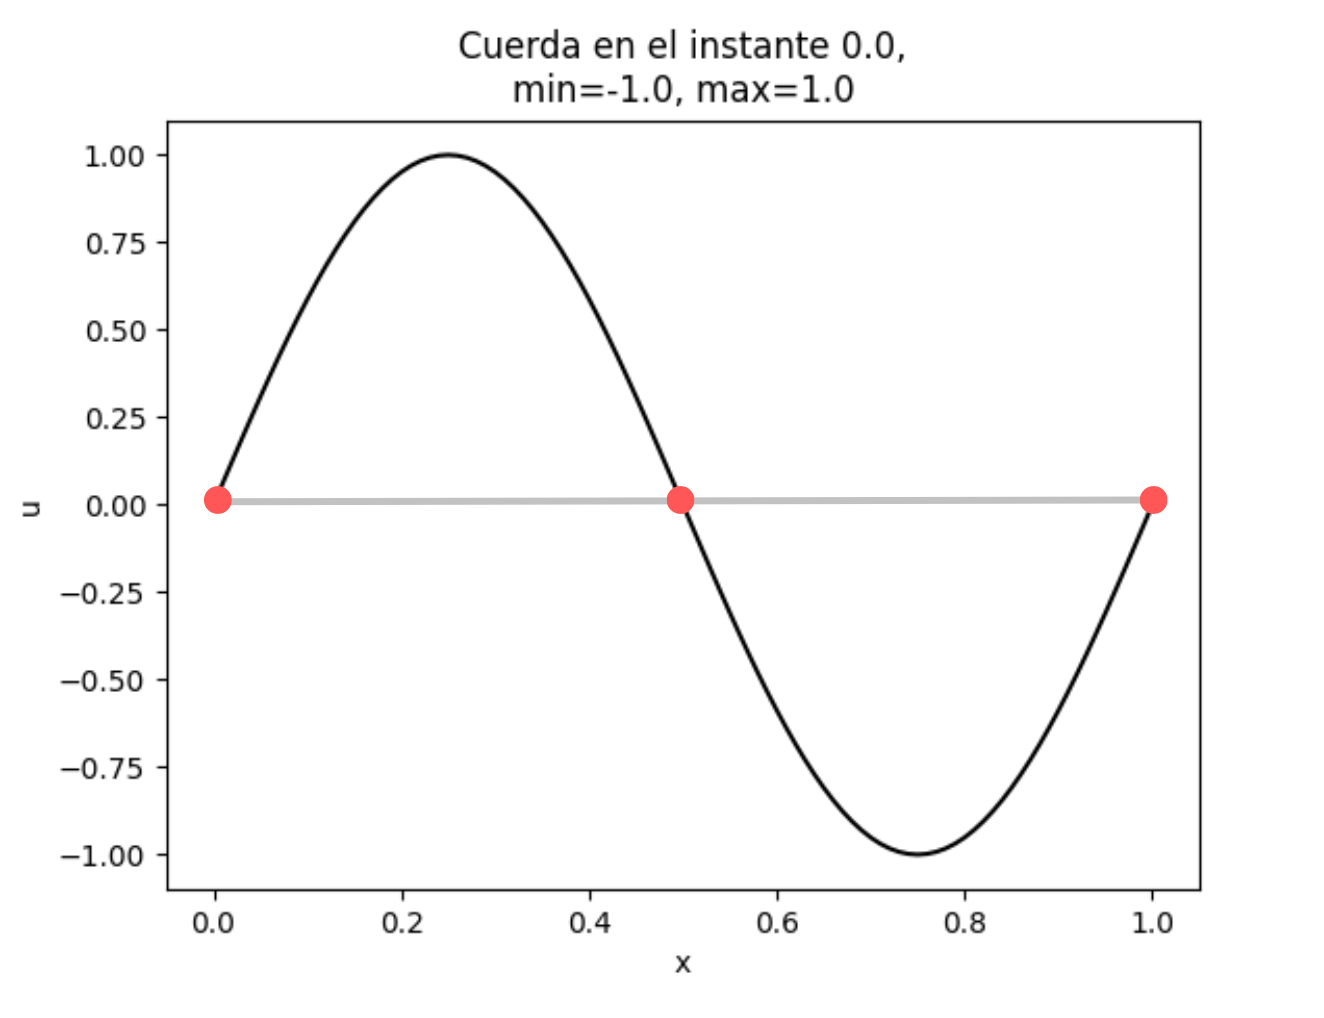
\includegraphics[width=\textwidth]{2Seno1.png}
		\caption{Posici�n inicial.}
		\label{fig:2Seno1}
	\end{minipage}
	\hfill
	\begin{minipage}[b]{0.45\textwidth}
		\centering
 		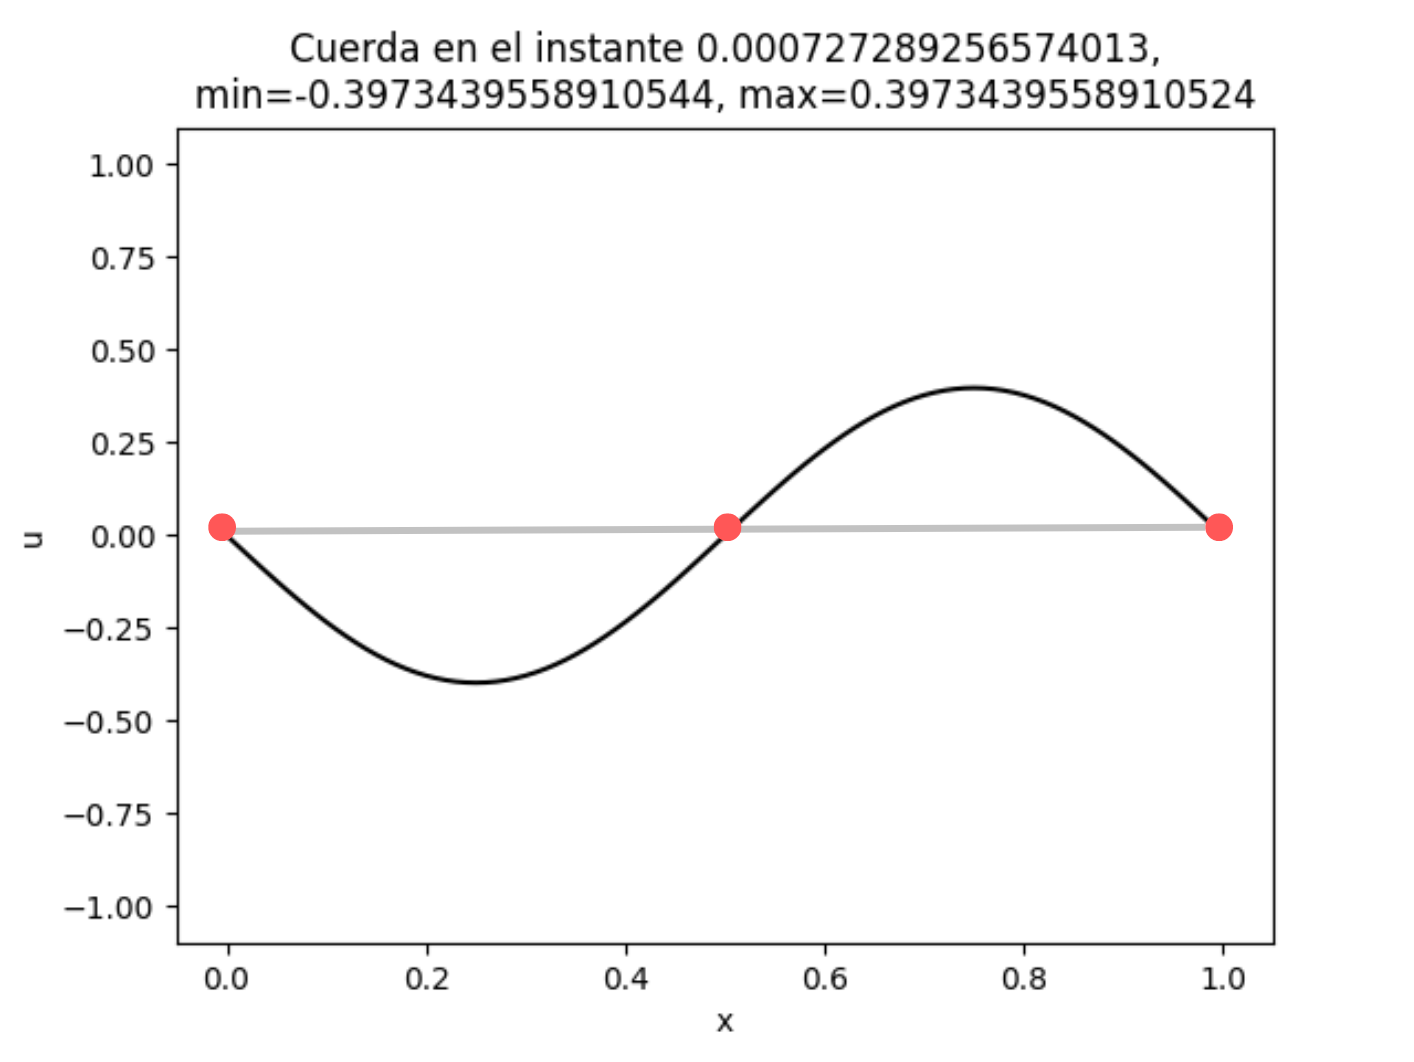
\includegraphics[width=\textwidth]{2Seno2.png}
		\caption{}
		\label{fig:2Seno2}
	\end{minipage}
\end{figure}

Podemos observar esto  eligiendo los puntos adecuados, $x=0.5$ y $x=0.25$, para seno de $\pi x$, \ref{subsec:sin(x)},  y seno de $2\pi x$. Vemos claramente que llega a su m�xima amplitud el doble de veces.

\begin{figure}[ht]
	\centering
	\begin{minipage}[b]{0.45\textwidth}
		\centering
		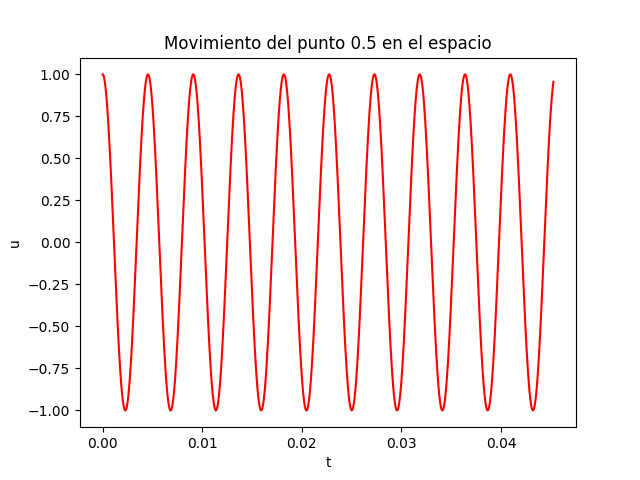
\includegraphics[width=\textwidth]{2Seno3.png}
		\caption{$sin(x)$ en $x=0.5$ Archivo figura5-5.wav}
		\label{fig:2Seno3}
	\end{minipage}
	\hfill
	\begin{minipage}[b]{0.45\textwidth}
		\centering
		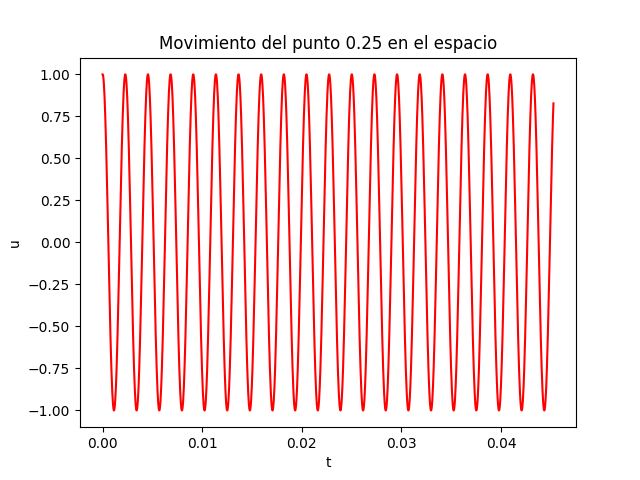
\includegraphics[width=\textwidth]{2Seno4.png}
		\caption{$sin(2x)$ en $x=0.25$ Archivo figura5-24.wav}
		\label{fig:2Seno4}
	\end{minipage}
\end{figure}

\section{Soluciones tipo onda viajera}
\label{sec:solondaviajera}

En esta secci�n nuestro objetivo ser� ejemplificar lo explicado en la secci�n  \ref{Ondaviajera}. Utilizando de nuevo la funci�n seno, las soluciones de tipo onda viajera en los siguientes casos ser�an:

\newpage
\begin{figure}[ht]
	\centering
	\begin{minipage}[b]{0.45\textwidth}
		\centering
		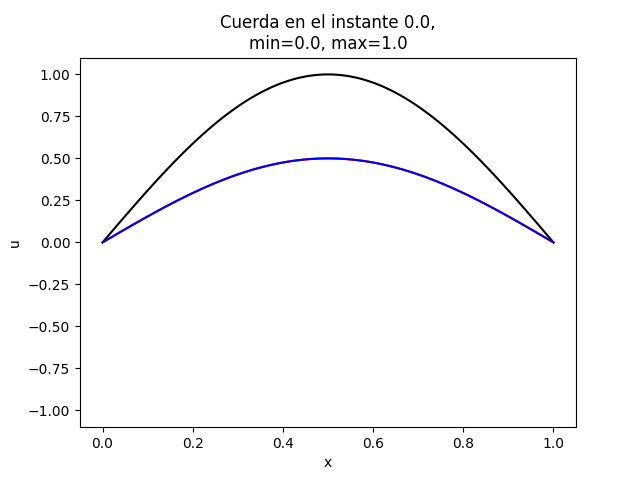
\includegraphics[width=\textwidth]{Senotrav1.png}
		\caption{Superpuestas ambas soluciones.\\$\ $\\ }
		\label{fig:Senotrav1}
	\end{minipage}
	\hfill
	\begin{minipage}[b]{0.45\textwidth}
		\centering
		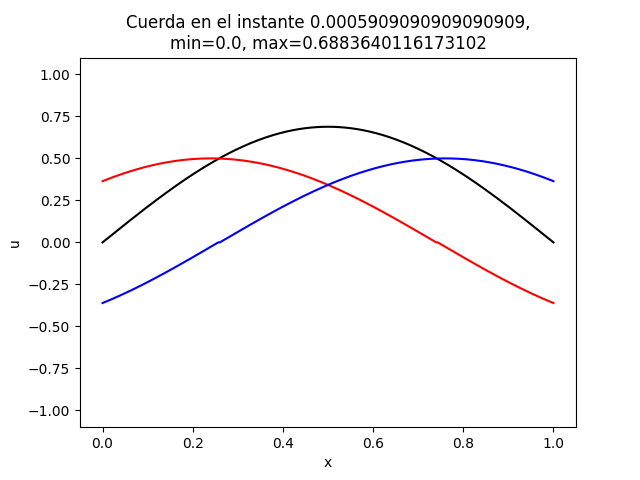
\includegraphics[width=\textwidth]{Senotrav2.png}
		\caption{Coloreada de azul la soluci�n que se desplaza a la derecha y de rojo la que se desplaza hacia la izquierda.}
		\label{fig:Senotrav2}
	\end{minipage}
\end{figure}

\vspace{2cm}

\begin{wrapfigure}[5]{r}{0.45\textwidth}
	\vspace{-2.5cm}
	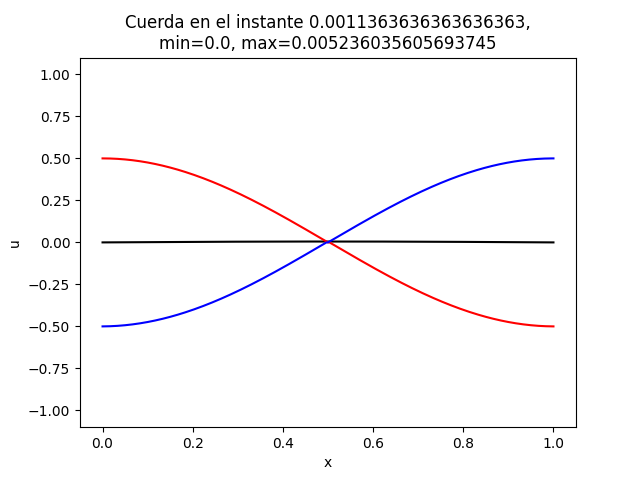
\includegraphics[width=0.45\textwidth]{Senotrav3.png}
	\caption{Movimiento de las soluciones de tipo onda viajera. }
	\label{fig:Senotrav3}
	
\end{wrapfigure}

Comprobamos que la suma de ambas soluciones nos da la posici�n de la cuerda en cada instante, coloreada de negro.\\

\vspace{1.5cm}
Esto se comprueba de manera incluso m�s clara con la funci�n $sen(2\pi x)$.

\begin{figure}[ht]
	\centering
	\begin{minipage}[b]{0.45\textwidth}
		\centering
		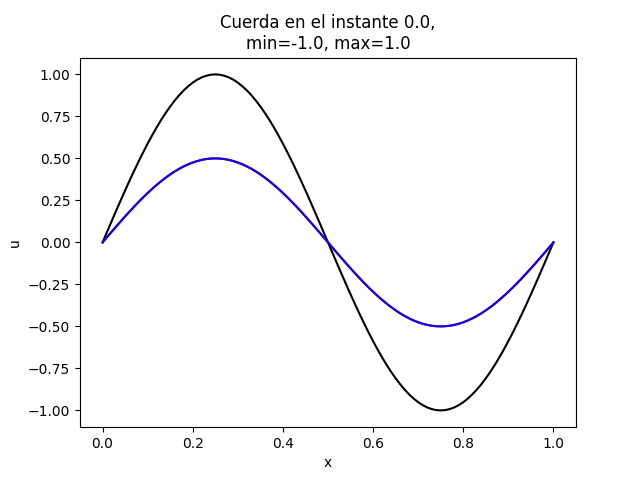
\includegraphics[width=\textwidth]{Senotrav4.png}
		\caption{}
		\label{fig:Senotrav4}
	\end{minipage}
	\hfill
	\begin{minipage}[b]{0.45\textwidth}
		\centering
		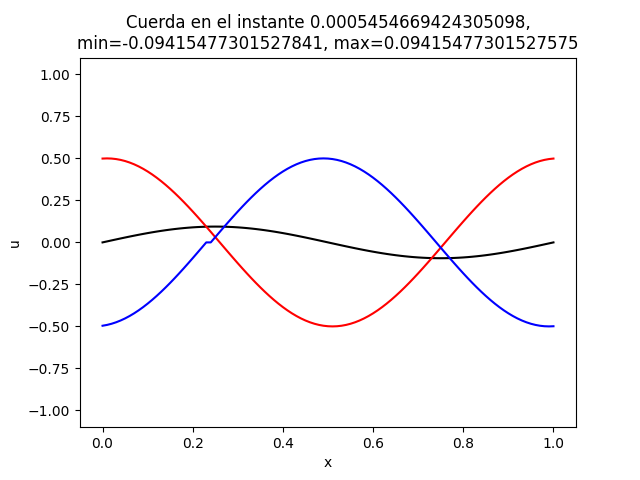
\includegraphics[width=\textwidth]{Senotrav6.png}
		\caption{}
		\label{fig:Senotrav5}
	\end{minipage}
\end{figure}
\newpage

\section{Comparac�n variando el valor de $\mu$}
Ahora veremos como cambiando el par�metro $\mu$, las soluciones obtenidas propagar�n inestabilidades.

\subsection{$\mu\ll 1$}
Cuando elegimos $\mu$ mucho menor que $1$, es decir, alej�ndonos de la soluci�n �ptima, poco a poco comienzan a generarse inestabilidades. Comparemos la soluci�n con $\mu = 1$, para $f(x)$ de tipo Struck.

\begin{figure}[ht]
	\centering
	\begin{minipage}[b]{0.45\textwidth}
		\centering
		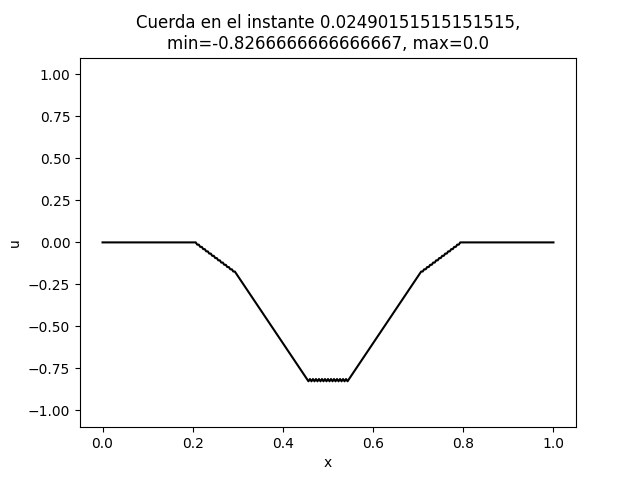
\includegraphics[width=\textwidth]{Piconormal.png}
		\caption{Soluci�n para $\mu=1$.}
		\label{fig:Piconormal}
	\end{minipage}
	\hfill
	\begin{minipage}[b]{0.45\textwidth}
		\centering
		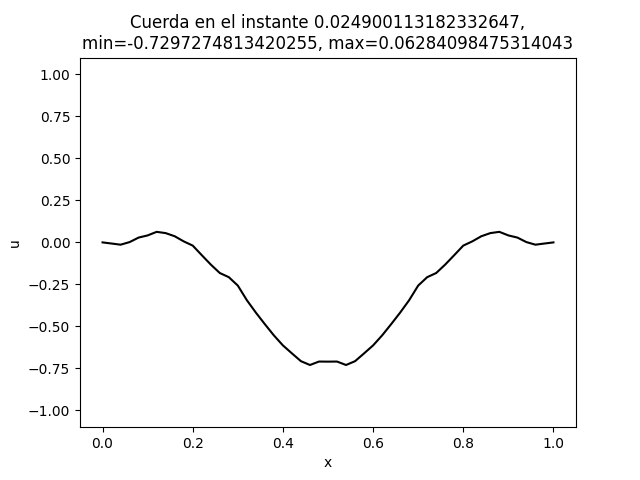
\includegraphics[width=\textwidth]{Picomu0.1.png}
		\caption{Soluci�n para $\mu=0.1$.}
		\label{fig:Picomu0.1}
	\end{minipage}
\end{figure}
En la imagen de la derecha podemos observar las inestabilidades en forma de ondas por toda la cuerda. Por otro lado, vemos claramente las diferencias en las im�genes del movimiento de la onda dependiendo del tiempo, con  el punto $x=0.5$ fijado.

\begin{figure}[ht]
	\centering
	\begin{minipage}[b]{0.45\textwidth}
		\centering
		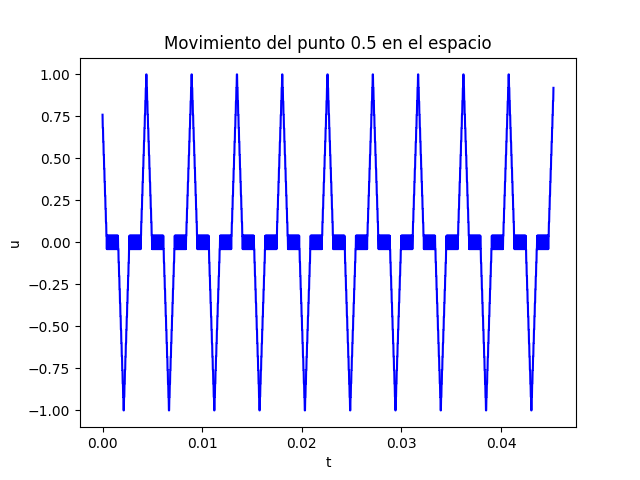
\includegraphics[width=\textwidth]{Picoondamu1.png}
		\caption{Movimiento de la onda para $\mu=1$. Archivo figura5-32.wav}
		\label{fig:Picoonda}
	\end{minipage}
	\hfill
	\begin{minipage}[b]{0.45\textwidth}
		\centering
		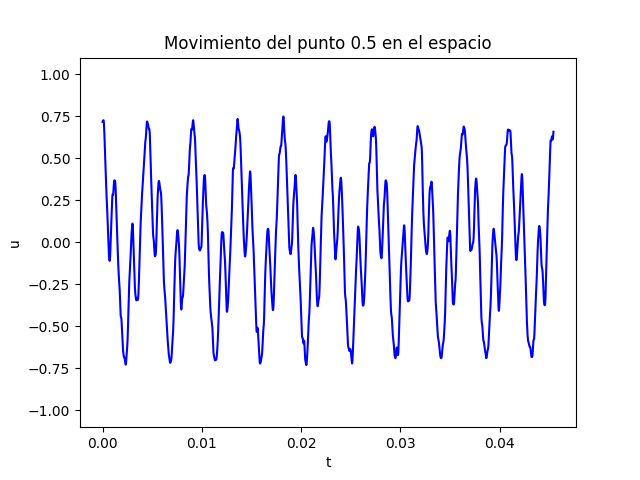
\includegraphics[width=\textwidth]{Picoondamu0.1.png}
		\caption{Movimiento de la onda para $\mu=0.1$. Archivo figura5-33.wav}
		\label{fig:Picoondamu0.1}
	\end{minipage}
\end{figure}
A�n viendo claramente las inestabilidades de forma gr�fica, no es tan f�cil escucharlas en los archivos de audio adjuntos.


\subsection{$\mu>1$}
Cuando violamos la condici�n CFL, las inestabilidades se propagar�n a�n m�s r�pido. Utilizando el mismo ejemplo que en el apartado anterior, podremos comprobar como se propagan a todos los puntos de la cuerda antes de llegar a los $0.002$ segundos.

\begin{figure}[ht]
	\centering
	\begin{minipage}[b]{0.45\textwidth}
		\centering
		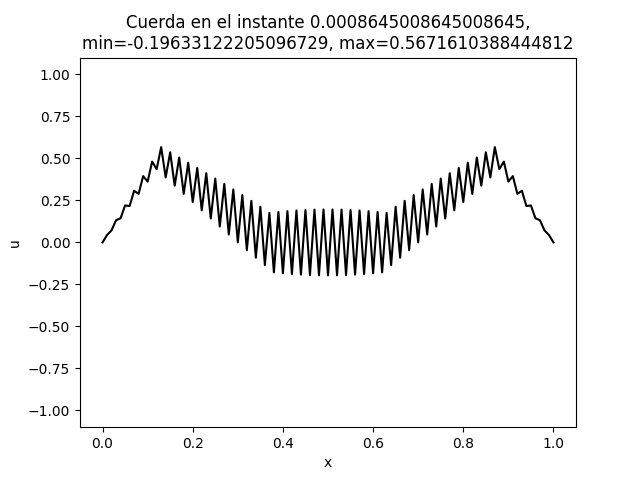
\includegraphics[width=\textwidth]{Pico38.png}
		\caption{Comienzo de las inestabilidades.}

	\end{minipage}
	\hfill
	\begin{minipage}[b]{0.45\textwidth}
		\centering
		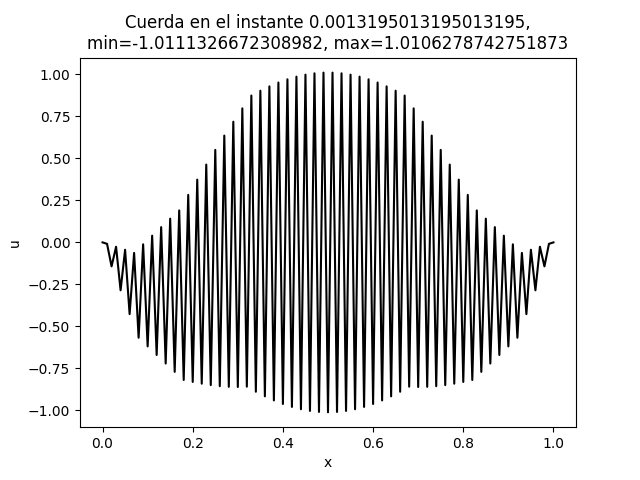
\includegraphics[width=\textwidth]{Pico58.png}
		\caption{Soluci�n para $\mu=0.1$.\\}
		\label{fig:Picomu1.1}
	\end{minipage}
\end{figure}
En este caso, a mayor sea $m$ antes se propagar�n las inestabilidades, por ello hemos elegido $m=40$, para observar como cambia la onda dependiendo del tiempo.

\begin{figure}[ht]
	\centering
	\begin{minipage}[b]{0.45\textwidth}
		\centering
		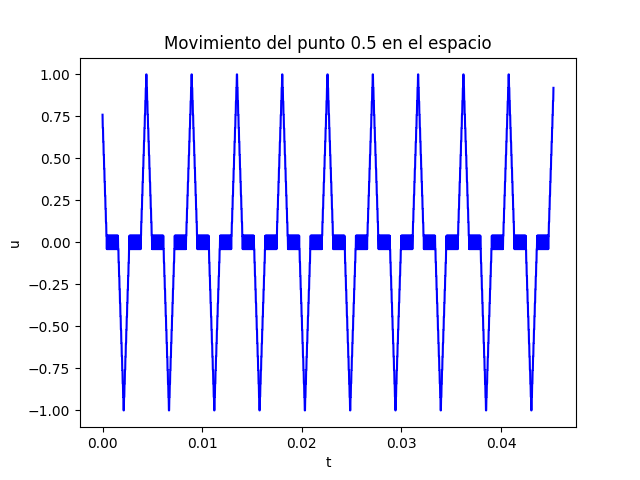
\includegraphics[width=\textwidth]{Picoondamu1.png}
		\caption{Movimiento de la onda para $\mu=1$.}
	\end{minipage}
	\hfill
	\begin{minipage}[b]{0.45\textwidth}
		\centering
		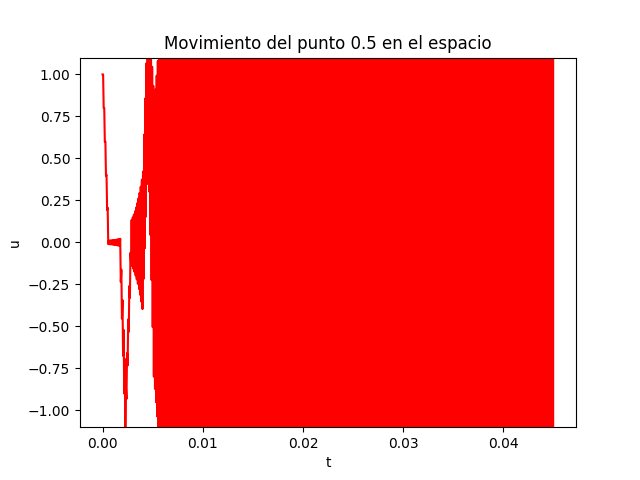
\includegraphics[width=\textwidth]{Picoondamu1.1.png}
		\caption{Movimiento de la onda para $\mu=0.1$. Archivo fig5-38.wav}
		\label{fig:Picoondamu1.1}
	\end{minipage}
\end{figure}
\newpage

Si intentamos reproducir el sonido de esta �ltima situaci�n no se escuchar� nada, puesto que las inestabilidades son tan grandes que hacen imposible su escucha, dos causas posibles son:
\begin{itemize}
	\item  El guardado en el formato .wav, puesto que cuando la amplitud es mayor que $1$, no lo capta de manera adecuada.
	\item La frecuencia, al ser tan elevada, es imposible de escuchar para el o�do humano.
\end{itemize}


\section{Comparar cambiando la energ�a}
\label{sec:ComparacionEnergia}
Cambio la energ�a y comparo 









% ----------------------------------------------------------------------

	

% Termina el trabajo con un capítulo de conclusiones, en el que puedes resolver algunos problemas, por ejemplo con los que empezaste, o con algunas generalizaciones del tema, ...
% !TeX encoding = ISO-8859-1
% !TeX encoding = ISO-8859-1

\chapter{Conclusiones y proyectos futuros }
\label{Conclusiones}
A lo largo de este trabajo, hemos introducido conceptos matem�ticos, tales como los espacios de Lebesgue y el producto interior, los hemos generalizado para el caso discreto, en un mallado definido para dicho ambiente. Ha sido fundamental definir distintos tipos de aproximaciones (progresivas, regresivas y centradas), que usadas adecuadamente nos llevan a esquemas num�ricos estables\\

Se ha contextualizado la ecuaci�n en derivadas parciales de onda, utilizando una perspectiva f�sica. Tambi�n se han analizado ciertas soluciones de la ecuaci�n, y la Ley de la conservaci�n de energ�a en la misma.\\

Una vez hecho esto, hemos examinado la soluci�n num�rica de la ecuaci�n de onda mediante el m�todo de las diferencias finitas, observando en \ref{sec:soluciones}, como se obtienen buenos resultados para la misma. Hemos comparado distintas condiciones iniciales que cumplen con los par�metros obtenidos mediante el an�lisis de Von Neumann \ref{sec:VonNeumann} y hemos conseguido archivos de audio que corroboran la estabilidad dentro del marco obtenido.\\

Por otro lado, hemos logrado la implementaci�n de las soluciones de tipo onda viajera \ref{sec:solondaviajera}, de las que derivamos que la suma de las mismas describe inequ�vocamente el movimiento de la cuerda del esquema estudiado.\\

A continuaci�n hemos representado la relaci�n entre la condici�n CFL y la inestabilidad de las soluciones, observando como su incumplimiento conduce a aproximaciones incorrectas, que llevan que presentan multitud de oscilaciones esp�reas.\\

En definitiva, hemos podido realizar un estudio general de la ecuaci�n de onda en derivadas parciales, abordando desde los conceptos fundamentales hasta la comprobaci�n de como las condiciones te�ricas son fundamentales para obtener una correcta soluci�n num�rica de la misma.\\

Este estudio ser�a f�cilmente ampliable tomando varios enfoques,

\begin{itemize}
	\item Utilizando argumentos similares a los encontrados en \cite{Optimal}, podr�amos hablar de la controlabilidad y observabilidad de nuestro esquema, en lugar de en un ambiente semi-discreto como el que propone Enrique Zuazua.
	\item Se podr�a enriquecer el estudio comparando diferentes esquemas usados asiduamente en el m�todo de las diferencias finitas, \citep{Russell, Optimal}.
	\item Tambi�n ser�a interesante estudiar si es adecuado el uso de m�todos de resoluci�n diferentes, como por ejemplo los m�todos espectrales, o elementos finitos \citep{Stig}.
	\item Considerar ecuaciones de ondas en dominios bidimensionales, como la piel de un tambor que vibra al ser golpeado por una baqueta.
	\item Un enfoque m�s aplicado que podr�amos abordar es, la utilizaci�n de los archivos .wav sintetizados para la creaci�n de m�sica, ya que hemos visto, que dependiendo de las condiciones iniciales, la forma de la onda obtenida cambia, de manera similar a como lo hace al tocar la misma nota en dos instrumentos diferentes.
	
\end{itemize}







% ----------------------------------------------------------------------

 	
	

% --------------------------------------------------------------
%:                  Partes finales: apéndices, bibliografía,..
% --------------------------------------------------------------

\backmatter


%: ----------------------- appendix ------------------------

% si tiene sentido en tu trabajo algún apéndice inclúyelo aquí

%\appendix


%: ----------------------- bibliografía ------------------------

% Muestra todas las entradas de la bibliografía no sólo las que son citadas en el trabajo
\nocite*

% Distintos estilos para la bibliografía:

\bibliographystyle{unsrt} % Defines the bibliography style
%\bibliographystyle{alpha} % Defines the bibliography style
%\bibliographystyle{apa-good} % Defines the bibliography style
%\bibliographystyle{natbib} % Defines the bibliography style
%\bibliographystyle{plainurl}

%%%%%%%%%%%%%%%%%%%%%%%%%%%%%%%%%%%%%%%%%%%%%%%%%%%%%%%
%%%%%%%   No olvides ejecutar BibTeX para la bibliografía cada vez que introduzcas algún artículo o libro
%%%%%%%%%%%%%%%%%%%%%%%%%%%%%%%%%%%%%%%%%%%%%%%%%%%%%%%%
\bibliography{bibliografia}



\end{document}
